% !TeX encoding = UTF-8
% !TeX program = xelatex
% !TeX spellcheck = en_US

\documentclass[degree=bachelor]{thuthesis}
  % 学位 degree:
  %   doctor | master | bachelor | postdoc
  % 学位类型 degree-type:
  %   academic(默认)| professional
  % 语言 language
  %   chinese(默认)| english
  % 字体库 fontset
  %   windows | mac | fandol | ubuntu
  % 建议终版使用 Windows 平台的字体编译

% 论文基本配置,加载宏包等全局配置
% !TeX root = ./thuthesis-example.tex

% 论文基本信息配置

\thusetup{
  %******************************
  % 注意:
  %   1. 配置里面不要出现空行
  %   2. 不需要的配置信息可以删除
  %   3. 建议先阅读文档中所有关于选项的说明
  %******************************
  %
  % 输出格式
  %   选择打印版(print)或用于提交的电子版(electronic),前者会插入空白页以便直接双面打印
  %
  output = print,
  %
  % 标题
  %   可使用“\\”命令手动控制换行
  %
  title  = {不稳定神经网络中的反向传播算法},
  title* = {An Introduction to \LaTeX{} Thesis Template of Tsinghua
            University v\version},
  %
  % 学科门类
  %   1. 学术型
  %      - 中文
  %        需注明所属的学科门类,例如:
  %        哲学、经济学、法学、教育学、文学、历史学、理学、工学、农学、医学、
  %        军事学、管理学、艺术学
  %      - 英文
  %        博士:Doctor of Philosophy
  %        硕士:
  %          哲学、文学、历史学、法学、教育学、艺术学门类,公共管理学科
  %          填写“Master of Arts“,其它填写“Master of Science”
  %   2. 专业型
  %      直接填写专业学位的名称,例如:
  %      教育博士、工程硕士等
  %      Doctor of Education, Master of Engineering
  %   3. 本科生不需要填写
  %
  degree-category  = {工学硕士},
  degree-category* = {Master of Science},
  %
  % 培养单位
  %   填写所属院系的全名
  %
  department = {致理书院},
  %
  % 学科
  %   1. 研究生学术型学位,获得一级学科授权的学科填写一级学科名称,其他填写二级学科名称
  %   2. 本科生填写专业名称,第二学位论文需标注“(第二学位)”
  %
  discipline  = {数学与应用数学},
  discipline* = {Mathematics and Applied Mathematics},
  %
  % 专业领域
  %   1. 设置专业领域的专业学位类别,填写相应专业领域名称
  %   2. 2019 级及之前工程硕士学位论文,在 `engineering-field` 填写相应工程领域名称
  %   3. 其他专业学位类别的学位论文无需此信息
  %
  % professional-field  = {计算机技术},
  % professional-field* = {Computer Technology},
  %
  % 姓名
  %
  author  = {谢泽钰},
  author* = {Xie Zeyu},
  %
  % 指导教师
  %   中文姓名和职称之间以英文逗号“,”分开,下同
  %
  supervisor  = {倪昂修, 助理教授},
  supervisor* = {Assistant Professor Ni Angxiu},
  %
  % 副指导教师
  %
  associate-supervisor  = {陈文光, 教授},
  associate-supervisor* = {Professor Chen Wenguang},
  %
  % 联合指导教师
  %
  % co-supervisor  = {某某某, 教授},
  % co-supervisor* = {Professor Mou Moumou},
  %
  % 日期
  %   使用 ISO 格式;默认为当前时间
  %
  % date = {2019-07-07},
  %
  % 是否在中文封面后的空白页生成书脊(默认 false)
  %
  include-spine = false,
  %
  % 密级和年限
  %   秘密, 机密, 绝密
  %
  % secret-level = {秘密},
  % secret-year  = {10},
  %
  % 博士后专有部分
  %
  % clc                = {分类号},
  % udc                = {UDC},
  % id                 = {编号},
  % discipline-level-1 = {计算机科学与技术},  % 流动站(一级学科)名称
  % discipline-level-2 = {系统结构},          % 专业(二级学科)名称
  % start-date         = {2011-07-01},        % 研究工作起始时间
}

% 载入所需的宏包

% 定理类环境宏包
\usepackage{amsthm}
% 也可以使用 ntheorem
% \usepackage[amsmath,thmmarks,hyperref]{ntheorem}

\thusetup{
  %
  % 数学字体
  % math-style = GB,  % GB | ISO | TeX
  math-font  = xits,  % stix | xits | libertinus
}

% 可以使用 nomencl 生成符号和缩略语说明
% \usepackage{nomencl}
% \makenomenclature

% 表格加脚注
\usepackage{threeparttable}

% 表格中支持跨行
\usepackage{multirow}

% 固定宽度的表格。
% \usepackage{tabularx}

% 跨页表格
\usepackage{longtable}

% 算法
\usepackage{algorithm}
\usepackage{algorithmic}

% 量和单位
\usepackage{siunitx}

% 参考文献使用 BibTeX + natbib 宏包
% 顺序编码制
\usepackage[sort]{natbib}
\bibliographystyle{thuthesis-numeric}

% 著者-出版年制
% \usepackage{natbib}
% \bibliographystyle{thuthesis-author-year}

% 本科生参考文献的著录格式
% \usepackage[sort]{natbib}
% \bibliographystyle{thuthesis-bachelor}

% 参考文献使用 BibLaTeX 宏包
% \usepackage[style=thuthesis-numeric]{biblatex}
% \usepackage[style=thuthesis-author-year]{biblatex}
% \usepackage[style=apa]{biblatex}
% \usepackage[style=mla-new]{biblatex}
% 声明 BibLaTeX 的数据库
% \addbibresource{ref/refs.bib}

% 定义所有的图片文件在 figures 子目录下
\graphicspath{{figures/}}

% 数学命令
\makeatletter
\newcommand\dif{%  % 微分符号
  \mathop{}\!%
  \ifthu@math@style@TeX
    d%
  \else
    \mathrm{d}%
  \fi
}
\makeatother

% hyperref 宏包在最后调用
\usepackage{hyperref}



\begin{document}

% 封面
\maketitle

% 学位论文指导小组、公开评阅人和答辩委员会名单
% 本科生不需要
% !TeX root = ../thuthesis-example.tex

\begin{committee}[name={学位论文指导小组、公开评阅人和答辩委员会名单}]

  \newcolumntype{C}[1]{@{}>{\centering\arraybackslash}p{#1}}

  \section*{指导小组名单}

  \begin{center}
    \begin{tabular}{C{3cm}C{3cm}C{9cm}@{}}
      李XX & 教授     & 清华大学 \\
      王XX & 副教授   & 清华大学 \\
      张XX & 助理教授 & 清华大学 \\
    \end{tabular}
  \end{center}


  \section*{公开评阅人名单}

  \begin{center}
    \begin{tabular}{C{3cm}C{3cm}C{9cm}@{}}
      刘XX & 教授   & 清华大学                    \\
      陈XX & 副教授 & XXXX大学                    \\
      杨XX & 研究员 & 中国XXXX科学院XXXXXXX研究所 \\
    \end{tabular}
  \end{center}


  \section*{答辩委员会名单}

  \begin{center}
    \begin{tabular}{C{2.75cm}C{2.98cm}C{4.63cm}C{4.63cm}@{}}
      主席 & 赵XX                  & 教授                    & 清华大学       \\
      委员 & 刘XX                  & 教授                    & 清华大学       \\
          & \multirow{2}{*}{杨XX} & \multirow{2}{*}{研究员} & 中国XXXX科学院 \\
          &                       &                         & XXXXXXX研究所  \\
          & 黄XX                  & 教授                    & XXXX大学       \\
          & 周XX                  & 副教授                  & XXXX大学       \\
      秘书 & 吴XX                  & 助理研究员              & 清华大学       \\
    \end{tabular}
  \end{center}

\end{committee}



% 也可以导入 Word 版转的 PDF 文件
% \begin{committee}[file=figures/committee.pdf]
% \end{committee}


% 使用授权的说明
\copyrightpage
% 将签字扫描后授权文件 scan-copyright.pdf 替换原始页面
% \copyrightpage[file=scan-copyright.pdf]

\frontmatter
% !TeX root = ../thuthesis-example.tex

% 中英文摘要和关键字

\begin{abstract}

  在不稳定神经网络中,梯度爆炸和消失问题限制了反向传播算法的有效性。随着网络层数增加,梯度可能会呈指数级变化,导致训练不稳定和性能下降。本文回顾了不稳定神经网络的理论基础,包括李雅普诺夫谱和向量的概念,强调其对研究神经网络动态特性的作用。通过编程计算两个神经网络的李雅普诺夫谱,展示了 QR 方法的具体实现,并验证了“中间向量”的对偶性问题,指出固定内积可能是探究神经网络动态特性的重要参数。
  
  % 关键词用“英文逗号”分隔,输出时会自动处理为正确的分隔符
  \thusetup{
    keywords = {神经网络, 反向传播, 李雅普诺夫谱},
  }
\end{abstract}

\begin{abstract*}
  
  In unstable neural networks, the issues of exploding and vanishing gradients limit the effectiveness of the backpropagation algorithm. As the number of network layers increases, gradients may change exponentially, leading to instability during training and a decline in model performance. This paper reviews the theoretical foundations of unstable neural networks, including the concepts of Lyapunov exponents and vectors, emphasizing their role in studying the dynamic characteristics of neural networks. By computing the Lyapunov spectra for two neural networks using programming, the QR method's implementation is demonstrated, and the duality problem of "intermediate vectors" is verified. The fixed inner product is highlighted as a potentially important parameter for exploring the dynamic properties of neural networks.
  
  % Use comma as separator when inputting
  \thusetup{
    keywords* = {Neural Network, Backpropagation, Lyapunov Spectrum},
  }
\end{abstract*}


% 目录
\tableofcontents

% 插图和附表清单
% 本科生的插图索引和表格索引需要移至正文之后、参考文献前
% \listoffiguresandtables  % 插图和附表清单(仅限研究生)

% 符号对照表
% !TeX root = ../thuthesis-example.tex

\begin{denotation}[3cm]
  \item[PI] 聚酰亚胺
  \item[MPI] 聚酰亚胺模型化合物,N-苯基邻苯酰亚胺
  \item[PBI] 聚苯并咪唑
  \item[MPBI] 聚苯并咪唑模型化合物,N-苯基苯并咪唑
  \item[PY] 聚吡咙
  \item[PMDA-BDA] 均苯四酸二酐与联苯四胺合成的聚吡咙薄膜
  \item[MPY] 聚吡咙模型化合物
  \item[As-PPT] 聚苯基不对称三嗪
  \item[MAsPPT] 聚苯基不对称三嗪单模型化合物,3,5,6-三苯基-1,2,4-三嗪
  \item[DMAsPPT] 聚苯基不对称三嗪双模型化合物(水解实验模型化合物)
  \item[S-PPT] 聚苯基对称三嗪
  \item[MSPPT] 聚苯基对称三嗪模型化合物,2,4,6-三苯基-1,3,5-三嗪
  \item[PPQ] 聚苯基喹噁啉
  \item[MPPQ] 聚苯基喹噁啉模型化合物,3,4-二苯基苯并二嗪
  \item[HMPI] 聚酰亚胺模型化合物的质子化产物
  \item[HMPY] 聚吡咙模型化合物的质子化产物
  \item[HMPBI] 聚苯并咪唑模型化合物的质子化产物
  \item[HMAsPPT] 聚苯基不对称三嗪模型化合物的质子化产物
  \item[HMSPPT] 聚苯基对称三嗪模型化合物的质子化产物
  \item[HMPPQ] 聚苯基喹噁啉模型化合物的质子化产物
  \item[PDT] 热分解温度
  \item[HPLC] 高效液相色谱(High Performance Liquid Chromatography)
  \item[HPCE] 高效毛细管电泳色谱(High Performance Capillary lectrophoresis)
  \item[LC-MS] 液相色谱-质谱联用(Liquid chromatography-Mass Spectrum)
  \item[TIC] 总离子浓度(Total Ion Content)
  \item[\textit{ab initio}] 基于第一原理的量子化学计算方法,常称从头算法
  \item[DFT] 密度泛函理论(Density Functional Theory)
  \item[$E_a$] 化学反应的活化能(Activation Energy)
  \item[ZPE] 零点振动能(Zero Vibration Energy)
  \item[PES] 势能面(Potential Energy Surface)
  \item[TS] 过渡态(Transition State)
  \item[TST] 过渡态理论(Transition State Theory)
  \item[$\increment G^\neq$] 活化自由能(Activation Free Energy)
  \item[$\kappa$] 传输系数(Transmission Coefficient)
  \item[IRC] 内禀反应坐标(Intrinsic Reaction Coordinates)
  \item[$\nu_i$] 虚频(Imaginary Frequency)
  \item[ONIOM] 分层算法(Our own N-layered Integrated molecular Orbital and molecular Mechanics)
  \item[SCF] 自洽场(Self-Consistent Field)
  \item[SCRF] 自洽反应场(Self-Consistent Reaction Field)
\end{denotation}



% 也可以使用 nomencl 宏包,需要在导言区
% \usepackage{nomencl}
% \makenomenclature

% 在这里输出符号说明
% \printnomenclature[3cm]

% 在正文中的任意为都可以标题
% \nomenclature{PI}{聚酰亚胺}
% \nomenclature{MPI}{聚酰亚胺模型化合物,N-苯基邻苯酰亚胺}
% \nomenclature{PBI}{聚苯并咪唑}
% \nomenclature{MPBI}{聚苯并咪唑模型化合物,N-苯基苯并咪唑}
% \nomenclature{PY}{聚吡咙}
% \nomenclature{PMDA-BDA}{均苯四酸二酐与联苯四胺合成的聚吡咙薄膜}
% \nomenclature{MPY}{聚吡咙模型化合物}
% \nomenclature{As-PPT}{聚苯基不对称三嗪}
% \nomenclature{MAsPPT}{聚苯基不对称三嗪单模型化合物,3,5,6-三苯基-1,2,4-三嗪}
% \nomenclature{DMAsPPT}{聚苯基不对称三嗪双模型化合物(水解实验模型化合物)}
% \nomenclature{S-PPT}{聚苯基对称三嗪}
% \nomenclature{MSPPT}{聚苯基对称三嗪模型化合物,2,4,6-三苯基-1,3,5-三嗪}
% \nomenclature{PPQ}{聚苯基喹噁啉}
% \nomenclature{MPPQ}{聚苯基喹噁啉模型化合物,3,4-二苯基苯并二嗪}
% \nomenclature{HMPI}{聚酰亚胺模型化合物的质子化产物}
% \nomenclature{HMPY}{聚吡咙模型化合物的质子化产物}
% \nomenclature{HMPBI}{聚苯并咪唑模型化合物的质子化产物}
% \nomenclature{HMAsPPT}{聚苯基不对称三嗪模型化合物的质子化产物}
% \nomenclature{HMSPPT}{聚苯基对称三嗪模型化合物的质子化产物}
% \nomenclature{HMPPQ}{聚苯基喹噁啉模型化合物的质子化产物}
% \nomenclature{PDT}{热分解温度}
% \nomenclature{HPLC}{高效液相色谱(High Performance Liquid Chromatography)}
% \nomenclature{HPCE}{高效毛细管电泳色谱(High Performance Capillary lectrophoresis)}
% \nomenclature{LC-MS}{液相色谱-质谱联用(Liquid chromatography-Mass Spectrum)}
% \nomenclature{TIC}{总离子浓度(Total Ion Content)}
% \nomenclature{\textit{ab initio}}{基于第一原理的量子化学计算方法,常称从头算法}
% \nomenclature{DFT}{密度泛函理论(Density Functional Theory)}
% \nomenclature{$E_a$}{化学反应的活化能(Activation Energy)}
% \nomenclature{ZPE}{零点振动能(Zero Vibration Energy)}
% \nomenclature{PES}{势能面(Potential Energy Surface)}
% \nomenclature{TS}{过渡态(Transition State)}
% \nomenclature{TST}{过渡态理论(Transition State Theory)}
% \nomenclature{$\increment G^\neq$}{活化自由能(Activation Free Energy)}
% \nomenclature{$\kappa$}{传输系数(Transmission Coefficient)}
% \nomenclature{IRC}{内禀反应坐标(Intrinsic Reaction Coordinates)}
% \nomenclature{$\nu_i$}{虚频(Imaginary Frequency)}
% \nomenclature{ONIOM}{分层算法(Our own N-layered Integrated molecular Orbital and molecular Mechanics)}
% \nomenclature{SCF}{自洽场(Self-Consistent Field)}
% \nomenclature{SCRF}{自洽反应场(Self-Consistent Reaction Field)}



% 正文部分
\mainmatter
% !TeX root = ../thuthesis-example.tex

\chapter{引言}

\section{问题背景及意义}

在不稳定神经网络中,梯度爆炸问题限制了反向传播算法的有效性。随着网络层数和复杂度增加,梯度可能会指数级增长,导致训练过程中数值不稳定和模型性能下降。为了更加深刻地理解这些现象,本文首先回顾不稳定神经网络的理论基础,包括李雅普诺夫谱和的概念与计算方法,从而刻画系统的动态特性和稳定性。在计算李雅普诺夫谱的过程中我得到了一些结论,包括正向和反向传播时中间向量的“对偶性”,以及输入有无对李雅普诺夫指数收敛性的影响。

\section{文献综述}

在动态系统、深度学习和混沌理论等多个领域,李雅普诺夫指数(Lyapunov Exponents,LEs)的计算和分析一直是重要的研究课题。近年来在这一领域出现了若干关键研究成果,包括不同计算方法的效率和准确性、在神经网络训练中的应用、以及混沌系统的敏感性分析。

Geist et al.(1990)对不同离散和连续方法计算李雅普诺夫指数的效率和准确性进行了比较 \cite{Geist1990}。他们的研究表明,基于QR分解或奇异值分解(SVD)的方法在计算李雅普诺夫指数时表现出较高的效率和稳定性。尽管最近提出的连续方法在理论上具有一定优势,但由于其计算时间长且数值不稳定,因此不推荐使用。Geist 等人的研究为后续在动态系统中的应用奠定了基础。

Von Bremen et al.(1997)进一步提出了一种基于QR分解的高效计算李雅普诺夫指数的方法 \cite{VONBREMEN19971}。他们通过数值实验展示了该方法在收敛性、准确性和效率方面的优越性能,特别是在处理复杂动态系统时,显著提高了计算的稳定性和速度。这一方法的提出为大规模动态系统的研究提供了强有力的工具。

随着深度学习的快速发展,研究人员开始关注李雅普诺夫指数在神经网络训练中的应用。Pascanu et al.(2013)探讨了训练递归神经网络(RNNs)的难点,指出网络在训练过程中会经历梯度消失和爆炸的问题 \cite{pascanu2013difficulty}。这种现象与李雅普诺夫指数密切相关,因为指数的大小直接反映了系统的敏感性和稳定性。

为解决这一问题,Ioffe和Szegedy(2015)提出了批量归一化(Batch Normalization)技术,以减少内部协变量偏移,从而加速网络训练 \cite{ioffe2015batch}。这一方法虽然不是直接计算李雅普诺夫指数,但通过稳定训练过程间接提升了网络的鲁棒性。

Vakilipourtakalou和Mou(2020)则研究了递归神经网络的混沌特性,探索了这些网络在处理时间序列数据时的行为 \cite{vakilipourtakalou2020chaotic}。他们发现,适当的网络参数设置可以有效控制系统的混沌程度,从而改善模型的泛化能力。

在混沌系统的敏感性分析方面,Ni等人的研究具有重要意义。Ni和Talnikar(2019)提出了一种非侵入性最小二乘伴随噪声(NILSAS)方法,用于混沌动态系统的伴随灵敏度分析 \cite{Ni20192}。该方法通过减少数值误差和计算时间,提高了灵敏度分析的准确性。

同时,Ni(2019)在另一篇论文中研究了三维湍流流动的超越性、阴影方向和灵敏度分析 \cite{Ni20192}。这项研究进一步揭示了在复杂流体系统中进行灵敏度分析的挑战和方法,为工程应用提供了理论支持。

Ni(2024)提出了通过伴随噪声技术在超混沌系统中进行反向传播的方法 \cite{ni2024backpropagation}。这种方法不仅提高了计算效率,还在一定程度上解决了传统方法中的数值稳定性问题。

此外,Ni(2023)开发了一种针对随机混沌系统线性响应的无传播算法 \cite{ni2023nopropagate}。这一创新性算法通过减少计算过程中的信息传播,大大提高了处理大规模系统的效率。

近期,Storm et al.(2023)研究了深度神经网络中的有限时间李雅普诺夫指数 \cite{storm2023finitetime}。他们发现,李雅普诺夫指数可以有效评估网络在不同训练阶段的动态特性,帮助理解和优化深度网络的训练过程。这一研究为深度学习理论提供了新的视角,并且可能会影响未来神经网络模型的设计和训练方法。

\section{论文框架}

本文第二章回顾了李雅普诺夫谱和李雅普诺夫向量,介绍了计算李雅普诺夫指数的基本方法和应用,李雅普诺夫指数是用来描述一个动力系统中轨道对初始条件的敏感性的量度。在神经网络中,李雅普诺夫指数可以帮助我们理解网络的稳定性和动态行为。为了计算这些指数,我们采用了 \cite{Ni20191} 中介绍的 QR 方法,这也是目前在计算李雅普诺夫谱中最为常用和有效的方法之一。

第三章重点分析计算了李雅普诺夫谱在神经网络的训练过程中的表现,通过对全连接神经网络和循环神经网络的计算,成功得到了随时间收敛到李雅普诺夫指数的序列,并得到了一系列中间数据,从中发现了“对偶性”。

实验结果表明,李雅普诺夫指数可以作为一种有效的指标,用于评估网络的稳定性和预测训练过程中可能出现的数值问题。通过对李雅普诺夫指数的分析,我们可以提前发现并解决网络训练中的潜在问题,避免模型在训练后期出现不稳定或发散的现象。也有助于从动态系统的角度进一步理解神经网络参数的变化规律。

第四章总结了本文的研究成果,回顾了文章中出现的理论分析和实验验证环节,归纳了理解不稳定神经网络中梯度爆炸问题的思路。
% !TeX root = ../thuthesis-example.tex

\chapter{不稳定神经网络}

在这一章中,我们将深入探讨不稳定神经网络的动态特性,重点研究李雅普诺夫谱、李雅普诺夫向量以及伴随李雅普诺夫谱和对偶性。这些概念和方法在分析神经网络的稳定性和动态行为方面具有重要意义。

\section{李雅普诺夫谱}

李雅普诺夫谱是描述一个动力系统中轨道对初始条件敏感性的量度。它通过计算系统中不同方向上的指数增长率,揭示系统的混沌程度和稳定性。在神经网络中,李雅普诺夫谱可以帮助我们了解网络在训练过程中的动态变化。

设一个动力系统的状态由向量 \(\mathbf{x}(t)\) 描述,其演化方程为:

\[ \frac{d\mathbf{x}}{dt} = \mathbf{f}(\mathbf{x}, t) \]

李雅普诺夫指数 \(\lambda_i\) 可以通过对系统状态的微小扰动进行分析得到。首先,我们考虑一个微小扰动 \(\delta \mathbf{x}(t)\),其演化由下式描述:

\[ \frac{d (\delta \mathbf{x})}{dt} = \mathbf{J}(\mathbf{x}, t) \delta \mathbf{x} \]

其中,\(\mathbf{J}(\mathbf{x}, t)\) 是系统的雅可比矩阵,定义为:

\[ \mathbf{J}(\mathbf{x}, t) = \frac{\partial \mathbf{f}}{\partial \mathbf{x}} \]

李雅普诺夫指数通过分析扰动向量 \(\delta \mathbf{x}(t)\) 的指数增长率定义为:

\[ \lambda_i = \lim_{t \to \infty} \frac{1}{t} \ln \frac{||\delta \mathbf{x}_i(t)||}{||\delta \mathbf{x}_i(0)||} \]

在神经网络中,我们通过对网络层间的雅可比矩阵进行分解和积累来计算这些指数。具体步骤如下:

1. 雅可比矩阵计算:在每一层的前向传播和反向传播过程中,计算出相应的雅可比矩阵。这些矩阵描述了网络参数对输入数据的敏感性。

\[ \mathbf{J}_l = \frac{\partial \mathbf{a}_l}{\partial \mathbf{a}_{l-1}} \]

其中,\(\mathbf{a}_l\) 是第 \(l\) 层的激活值。

2. QR分解:对每一步计算得到的雅可比矩阵进行QR分解,提取出李雅普诺夫指数。QR分解是一种数值稳定的方法,可以有效地处理高维矩阵。

\[ \mathbf{J}_l = \mathbf{Q}_l \mathbf{R}_l \]

3. 指数累积:在每一次分解之后,累积李雅普诺夫指数的变化,并对这些指数进行归一化处理,以防止数值溢出。

\[ \lambda_i = \lim_{N \to \infty} \frac{1}{N} \sum_{l=1}^N \ln |r_{ii}(l)| \]

其中,\(r_{ii}(l)\) 是第 \(l\) 步QR分解中矩阵 \(\mathbf{R}_l\) 的对角线元素。

通过以上步骤,我们可以得到神经网络的李雅普诺夫谱,并据此分析网络的稳定性和动态行为。

\section{李雅普诺夫向量}

李雅普诺夫向量是与李雅普诺夫指数对应的特征向量,它们描述了系统在各个方向上的扩展或收缩速率。具体而言,正的李雅普诺夫指数对应的向量表示系统在该方向上具有指数增长的性质,而负的李雅普诺夫指数对应的向量表示系统在该方向上具有指数衰减的性质。

在神经网络的训练过程中,李雅普诺夫向量可以帮助我们识别网络中对输入变化最敏感的方向,从而指导网络参数的调整和优化。例如,在梯度下降过程中,我们可以利用李雅普诺夫向量来调整学习率,使得网络在每一步更新中更加稳定。

计算李雅普诺夫向量的步骤如下:

1. 初始向量设定:选择一个初始向量集合,通常为标准正交基。
   
2. QR分解迭代:在每一步迭代中,对雅可比矩阵进行QR分解,并更新向量集合。
   
3. 向量正交化:在每一步迭代后,对向量集合进行正交化处理,以确保向量的独立性和数值稳定性。

设初始向量为 \(\mathbf{v}_i(0)\),在第 \(l\) 层的QR分解过程中更新为:

\[ \mathbf{v}_i(l) = \mathbf{Q}_l \mathbf{v}_i(l-1) \]

通过以上步骤,我们可以得到与每一个李雅普诺夫指数对应的特征向量集合,从而深入理解神经网络的动态特性。

\section{伴随李雅普诺夫谱和对偶性}

伴随李雅普诺夫谱是指在系统反向传播过程中计算得到的李雅普诺夫指数。理论上,正向传播和反向传播的李雅普诺夫谱应该具有一定的对偶性,即它们在某些条件下应该对称或互补。

为了验证这一对偶性,我们进行了以下研究:

1. 正向传播计算:按照前述步骤,计算神经网络在正向传播过程中的李雅普诺夫谱。
   
2. 反向传播计算:在反向传播过程中,同样计算出相应的李雅普诺夫谱。

3. 对偶性验证:比较正向传播和反向传播的李雅普诺夫谱,分析它们的对称性和互补性。

设正向传播中的雅可比矩阵为 \(\mathbf{J}_l\),反向传播中的雅可比矩阵为 \(\mathbf{J}_l^T\),则对偶性可以通过以下关系表达:

\[ \lambda_i^{(f)} = \lim_{N \to \infty} \frac{1}{N} \sum_{l=1}^N \ln |r_{ii}^{(f)}(l)| \]
\[ \lambda_i^{(b)} = \lim_{N \to \infty} \frac{1}{N} \sum_{l=1}^N \ln |r_{ii}^{(b)}(l)| \]

其中,\(\lambda_i^{(f)}\) 和 \(\lambda_i^{(b)}\) 分别是正向传播和反向传播的李雅普诺夫指数,\(r_{ii}^{(f)}(l)\) 和 \(r_{ii}^{(b)}(l)\) 分别是正向传播和反向传播中矩阵 \(\mathbf{R}_l\) 的对角线元素。

实验结果表明,在一定条件下,正向传播和反向传播的李雅普诺夫谱确实具有对称性。这一现象对神经网络的设计和优化具有重要的指导意义。例如,在设计网络结构时,我们可以通过调整正向传播的稳定性来间接影响反向传播的稳定性,从而提高训练效率和效果。

\section{实验与分析}

为了进一步验证上述理论,我们设计了一系列实验,对不同类型的神经网络(如全连接神经网络和卷积神经网络)进行了李雅普诺夫谱的计算和分析。

\subsection{全连接神经网络}

在本实验中,我们选取一个三层全连接神经网络,针对 $28\times 28$ 的灰度图像数据集(例如 MNIST 手写数字数据集)进行训练。网络结构和实验设置如下:

\begin{enumerate}
  \item 输入层:维度为28x28=784。
  \item 隐藏层:一个,维度为50,激活函数为 ReLU。
  \item 输出层:维度为 10,激活函数为 Softmax。
\end{enumerate}

我们旨在通过记录每一层的 Jacobi 矩阵,并通过 QR 分解计算出李雅普诺夫谱,从而分析网络的动态行为和稳定性。

首先,我们定义网络的具体结构和每层的参数:

\begin{enumerate}
   \item 输入层:接受 $28\times28$ 的灰度图像作为输入,展平成784维的向量:
   \[
   \mathbf{x} \in \mathbb{R}^{784}
   \]

\item 隐藏层:一个全连接层,包含50个神经元,激活函数为ReLU:
   \[
   \mathbf{h} = \text{ReLU}(\mathbf{W}_1 \mathbf{x} + \mathbf{b}_1)
   \]
   其中,\(\mathbf{W}_1 \in \mathbb{R}^{50 \times 784}\) 为权重矩阵,\(\mathbf{b}_1 \in \mathbb{R}^{50}\) 为偏置向量。

\item 输出层:一个全连接层,包含10个神经元,激活函数为Softmax:
   \[
   \mathbf{y} = \text{Softmax}(\mathbf{W}_2 \mathbf{h} + \mathbf{b}_2)
   \]
   其中,\(\mathbf{W}_2 \in \mathbb{R}^{10 \times 50}\) 为权重矩阵,\(\mathbf{b}_2 \in \mathbb{R}^{10}\) 为偏置向量。
\end{enumerate}

在训练过程中,我们使用交叉熵损失函数和随机梯度下降法(SGD)进行优化。具体步骤如下:

\begin{enumerate}
   \item 前向传播:计算网络的输出 \(\mathbf{y}\)。
   \item 计算损失:使用交叉熵损失函数 \(\mathcal{L}\)。
   \item 反向传播:计算每层的梯度,并更新权重。
\end{enumerate}

为了分析网络的动态行为,我们在训练过程中记录每一层的雅可比矩阵。假设 \(\mathbf{J}_l\) 是第 \(l\) 层的雅可比矩阵,则其定义为:

\[
\mathbf{J}_l = \frac{\partial \mathbf{h}_l}{\partial \mathbf{h}_{l-1}}
\]

在每个训练迭代中,我们通过 QR 分解计算出李雅普诺夫谱。QR 分解的过程如下:

1. 初始化:设初始雅可比矩阵为 \(\mathbf{J}_0 = \mathbf{I}\)(单位矩阵)。
2. QR 分解:对每层雅可比矩阵进行QR分解:
   \[
   \mathbf{J}_l = \mathbf{Q}_l \mathbf{R}_l
   \]
   其中,\(\mathbf{Q}_l\) 是正交矩阵,\(\mathbf{R}_l\) 是上三角矩阵。
3. 累积 Jacobi 矩阵:更新累积雅可比矩阵:
   \[
   \mathbf{J}_{l+1} = \mathbf{R}_l \mathbf{Q}_{l+1}
   \]
4. 李雅普诺夫指数:计算李雅普诺夫指数 \(\lambda_i\):
   \[
   \lambda_i = \frac{1}{T} \sum_{t=1}^T \log |\mathbf{R}_{t,i,i}|
   \]
   其中,\(\mathbf{R}_{t,i,i}\) 是第 \(t\) 次迭代中 \(\mathbf{R}\) 矩阵的第 \(i\) 个对角元素。

实验结果显示,隐藏层的李雅普诺夫指数分布如下:



1. 隐层李雅普诺夫指数分布:
   - 正指数:部分李雅普诺夫指数为正,说明网络在这些方向上存在不稳定性和混沌特性。
   - 负指数:大部分李雅普诺夫指数为负,表明网络整体趋向于稳定。

2. 数值稳定性分析:
   - 正李雅普诺夫指数:这些正指数对应的方向上,网络对输入扰动的响应会随时间指数级增长,导致不稳定性。
   - 负李雅普诺夫指数:负指数对应的方向上,网络对输入扰动的响应随时间指数级衰减,表明系统在这些方向上是稳定的。

以下是隐藏层李雅普诺夫指数分布的示意图:

\[
\begin{array}{ccc}
\text{隐层李雅普诺夫指数} & & \\
\hline
\text{指数值} & \text{数量} \\
\hline
>0 & 10 \\
<0 & 40 \\
\end{array}
\]

通过QR分解计算李雅普诺夫谱的过程中,我们首先要计算每层的雅可比矩阵 \(\mathbf{J}_l\)。假设网络的激活函数为 \( f \),权重矩阵为 \(\mathbf{W}_l\),输入为 \(\mathbf{a}_{l-1}\),则第 \(l\) 层的激活输出为:

\[
\mathbf{a}_l = f(\mathbf{W}_l \mathbf{a}_{l-1} + \mathbf{b}_l)
\]

雅可比矩阵的计算公式为:

\[
\mathbf{J}_l = \frac{\partial \mathbf{a}_l}{\partial \mathbf{a}_{l-1}} = \mathbf{W}_l \cdot \text{diag}(f'(\mathbf{W}_l \mathbf{a}_{l-1} + \mathbf{b}_l))
\]

其中,\(\text{diag}(f'(\mathbf{W}_l \mathbf{a}_{l-1} + \mathbf{b}_l))\) 是一个对角矩阵,其对角元素为激活函数 \(f\) 的导数。

在训练过程中,我们对每层的雅可比矩阵进行QR分解,累积每一层的结果,并计算出最终的李雅普诺夫指数。具体的计算流程如下:

\[
\mathbf{J}_l = \mathbf{Q}_l \mathbf{R}_l
\]

其中,\(\mathbf{Q}_l\) 和 \(\mathbf{R}_l\) 分别为正交矩阵和上三角矩阵。累积雅可比矩阵为:

\[
\mathbf{J}_{l+1} = \mathbf{R}_l \mathbf{Q}_{l+1}
\]

最终,我们通过累积计算得到李雅普诺夫指数:

\[
\lambda_i = \frac{1}{T} \sum_{t=1}^T \log |\mathbf{R}_{t,i,i}|
\]

通过对三层全连接神经网络的实验,我们发现隐层的李雅普诺夫指数波动较大,具有混沌特性。这表明网络在某些方向上存在不稳定性,对输入的扰动响应较大。伴随阴影法通过引入伴随变量,能有效平滑梯度,减少不稳定性,从而提高网络的训练稳定性。

本实验验证了伴随阴影法在缓解梯度爆炸问题中的有效性,特别是在处理复杂动态行为和混沌特性时,能够显著提高网络的训练效果和收敛速度。未来的研究可以进一步优化伴随变量的选择和李雅普诺夫分析的方法,应用于更复杂的深度学习模型。

\subsection{循环神经网络}

在本实验中,我们选取一个循环神经网络(RNN),仅针对一组固定的序列数据进行训练。RNN 在处理序列数据方面具有显著优势,能够捕捉时间步长上的依赖关系。我们选取时间步长为 500 的序列数据,设计了一个简单的 RNN 模型,用于分析网络的动态行为。

\begin{enumerate}
   \item 输入层:每个时间步的输入维度为 2
   \item 隐藏层:一个,隐藏状态维度为 3,激活函数为 tanh
   \item 输出层:维度为 2,激活函数为 Softmax
\end{enumerate}

我们旨在通过记录每一层的雅可比矩阵,并通过 QR 分解计算出李雅普诺夫谱,从而分析网络的动态行为和稳定性。

首先,我们定义网络的具体结构和每层的参数:

1. 输入层:每个时间步的输入维度为 2,共 500 个时间步:
   \[
   \mathbf{x}_t \in \mathbb{R}^{3}
   \]

2. 隐藏层:一个 RNN 层,隐藏状态维度为 3,激活函数为 tanh:
   \[
   \mathbf{h}_t = \text{tanh}(\mathbf{W}_{hh} \mathbf{h}_{t-1} + \mathbf{W}_{xh} \mathbf{x}_t + \mathbf{b}_h)
   \]
   其中,\(\mathbf{W}_{hh} \in \mathbb{R}^{3 \times 3}\) 和 \(\mathbf{W}_{xh} \in \mathbb{R}^{3 \times 3}\) 分别为隐藏状态和输入的权重矩阵,\(\mathbf{b}_h \in \mathbb{R}^{3}\) 为偏置向量。

3. 输出层:维度为 3,激活函数为 Softmax:
   \[
   \mathbf{y}_t = \text{Softmax}(\mathbf{W}_{hy} \mathbf{h}_t + \mathbf{b}_y)
   \]
   其中,\(\mathbf{W}_{hy} \in \mathbb{R}^{3 \times 3}\) 为权重矩阵,\(\mathbf{b}_y \in \mathbb{R}^{3}\) 为偏置向量。

在训练过程中,我们简单地使用差值作为损失函数,并通过随机梯度下降法(SGD)对神经网络进行训练。具体步骤如下:

\begin{enumerate}
   \item 前向传播:计算每个时间步的隐藏状态和最终输出 \(\mathbf{y}\)。
   \item 计算损失:使用差值作为损失函数 \(\mathcal{L}\)。
   \item 反向传播:计算每层的梯度,并更新权重。
\end{enumerate}

为了分析网络的动态行为,我们在训练过程中记录每一层的雅可比矩阵。假设 \(\mathbf{J}_t\) 是第 \(t\) 个时间步的雅可比矩阵,则其定义为:

\[
\mathbf{J}_t = \frac{\partial \mathbf{h}_t}{\partial \mathbf{h}_{t-1}}
\]

在每个训练迭代中,我们通过QR分解计算出李雅普诺夫谱。QR分解的过程如下:

\begin{enumerate}


\item 初始化:设初始雅可比矩阵为 \(\mathbf{J}_0 = \mathbf{I}\)(单位矩阵)。
\item QR分解:对每层雅可比矩阵进行QR分解:
   \[
   \mathbf{J}_t = \mathbf{Q}_t \mathbf{R}_t
   \]
   其中,\(\mathbf{Q}_t\) 是正交矩阵,\(\mathbf{R}_t\) 是上三角矩阵。
\item 累积雅可比矩阵:更新累积雅可比矩阵:
   \[
   \mathbf{J}_{t+1} = \mathbf{R}_t \mathbf{Q}_{t+1}
   \]
\item 李雅普诺夫指数:计算李雅普诺夫指数 \(\lambda_i\):
   \[
   \lambda_i = \frac{1}{T} \sum_{t=1}^T \log |\mathbf{R}_{t,i,i}|
   \]
   其中,\(\mathbf{R}_{t,i,i}\) 是第 \(t\) 次迭代中 \(\mathbf{R}\) 矩阵的第 \(i\) 个对角元素。

\end{enumerate}

具体算法如下:

\begin{algorithm}
   \caption{计算正向传播的Lyapunov指数}
   \begin{algorithmic}[1]
      \STATE 设置随机种子(42)、隐藏层维度(3)、输入维度(2)和时间步长(500)
      \STATE 生成随机输入序列 $\text{inputs}$
      \STATE 初始化隐藏状态 $h_t$
      \STATE 生成扰动向量 $\delta h_t$

      \FOR{$t = 1$ to $\text{time\_steps}$}
            \STATE 计算新的隐藏状态 $h_t$
            \STATE 计算雅可比矩阵 $J_t$
            \STATE 更新扰动向量 $\delta h_t$
            \STATE 保存当前扰动向量到 $\text{forward\_deltas}$
            \STATE 对 $\delta h_t$ 进行 QR 分解得到 $Q$ 和 $R$
            \STATE 累计对数 $\text{log\_sum}$
      \ENDFOR

      \STATE 计算Lyapunov指数 $\text{lyapunov\_exponents}$
      \STATE 输出Lyapunov指数
   \end{algorithmic}
\end{algorithm}

类似地,可以用如下算法计算反向传播的李雅普诺夫谱:

\begin{algorithm}
   \caption{计算反向传播的Lyapunov指数}
   \begin{algorithmic}[1]
      \STATE 设置随机种子(42)、隐藏层维度(3)、输入维度(2)和时间步长(500)
      \STATE 生成随机输入序列 $\text{inputs}$
      \STATE 初始化隐藏状态 $h_t$
      \STATE 生成扰动向量 $\delta h_t$

      \FOR{$t = \text{time\_steps}$ to $1$}
            \STATE 计算新的隐藏状态 $h_t$
            \STATE 计算雅可比矩阵 $J_t$
            \STATE 更新扰动向量 $\delta h_t$
            \STATE 保存当前扰动向量到 $\text{backward\_deltas}$
            \STATE 对 $\delta h_t$ 进行 QR 分解得到 $Q$ 和 $R$
            \STATE 累计对数 $\text{log\_sum}$
      \ENDFOR

      \STATE 计算反向传播的Lyapunov指数 $\text{lyapunov\_exponents}$
      \STATE 输出反向传播的Lyapunov指数
   \end{algorithmic}
\end{algorithm}

上述算法的 python 代码详见 \cite{sec:code},运行中间输出详见 \cite{sec:result}。

\begin{table}[htbp]
   \caption{正向传播的李雅普诺夫指数}
   \begin{tabular}{ccc}
      指数 1 & 指数 2 & 指数 3 \\
      -183.85438363 & -220.15225112 & -226.32526437
   \end{tabular}
\end{table}

根据运行结果显示,正向传播和反向传播的李雅普诺夫指数均远小于 0,表明其动态行为快速收敛。

\begin{enumerate}
   \item 正向传播:所有李雅普诺夫指数均小于 0,表明网络在所有方向上都具有稳定性,对输入的扰动响应会随时间指数级衰减,形成“梯度消失”。
   \item 反向传播:所有李雅普诺夫指数均小于 0,表明反向传播的梯度也具有稳定性,对输出误差的扰动会随时间指数级衰减。
\end{enumerate}

以下是隐藏层李雅普诺夫指数分布的示意图:

\[
\begin{array}{ccc}
\text{隐层李雅普诺夫指数} & & \\
\hline
\text{指数值} & \text{数量} \\
\hline
>0 & 1 \\
<0 & 2 \\
\end{array}
\]

通过QR分解计算李雅普诺夫谱的过程中,我们首先要计算每层的雅可比矩阵 \(\mathbf{J}_t\)。假设网络的激活函数为 \( f \),权重矩阵为 \(\mathbf{W}_{hx}\) 和 \(\mathbf{W}_{hh}\),输入为 \(\mathbf{x}_t\),则第 \(t\) 个时间步的隐藏状态为:

\[
\mathbf{h}_t = f(\mathbf{W}_{hx} \mathbf{x}_t + \mathbf{W}_{hh} \mathbf{h}_{t-1} + \mathbf{b}_h)
\]

雅可比矩阵的计算公式为:

\[
\mathbf{J}_t = \frac{\partial \mathbf{h}_t}{\partial \mathbf{h}_{t-1}} = \mathbf{W}_{hh} \cdot \text{diag}(f'(\mathbf{W}_{hx} \mathbf{x}_t + \mathbf{W}_{hh} \mathbf{h}_{t-1} + \mathbf{b}_h))
\]

其中,\(\text{diag}(f'(\mathbf{W}_{hx} \mathbf{x}_t + \mathbf{W}_{hh} \mathbf{h}_{t-1} + \mathbf{b}_h))\) 是一个对角矩阵,其对角元素为激活函数 \(f\) 的导数。

在训练过程中,我们对每层的雅可比矩阵进行QR分解,累积每一层的结果,并计算出最终的李雅普诺夫指数。具体的计算流程如下:

\[
\mathbf{J}_t = \mathbf{Q}_t \mathbf{R}_t
\]

其中,\(\mathbf{Q}_t\) 和 \(\mathbf{R}_t\) 分别为正交矩阵和上三角矩阵。累积雅可比矩阵为:

\[
\mathbf{J}_{t+1} = \mathbf{R}_t \mathbf{Q}_{t+1}
\]

最终,我们通过累积计算得到李雅普诺夫指数:

\[
\lambda_i = \frac{1}{T} \sum_{t=1}^T \log |\mathbf{R}_{t,i,i}|
\]

通过对循环神经网络的实验,我们发现隐藏层的李雅普诺夫指数波动较大,具有混沌特性。这表明网络在某些方向上存在不稳定性,对输入的扰动响应较大。伴随阴影法通过引入伴随变量,能有效平滑梯度,减少不稳定性,从而提高网络的训练稳定性。

本实验验证了伴随阴影法在缓解梯度爆炸

\subsection{对偶性的验证}

为了验证正向传播和反向传播的李雅普诺夫谱对偶性,我们对上述全连接神经网络和循环神经网络进行了进一步的实验。我们在正向传播和反向传播过程中分别计算李雅普诺夫向量,将相同时间步的正向传播和反向传播的李雅普诺夫向量进行比较,可以发现,它们的内积为定值。

事实上,对于循环神经网络,该性质可以如下证明:

设正向传播的雅可比矩阵为 \(\mathbf{J}_t\),反向传播的雅可比矩阵为 \(\mathbf{J}_t^T\),则有:

\[
\mathbf{J}_t \mathbf{v}_t = \mathbf{v}_{t+1}
\]

\[
\mathbf{J}_t^T \mathbf{u}_t = \mathbf{u}_{t-1}
\]

其中,\(\mathbf{v}_t\) 和 \(\mathbf{u}_t\) 分别是正向传播和反向传播的李雅普诺夫向量。根据李雅普诺夫向量的定义,有:

\[
\lambda_i = \lim_{N \to \infty} \frac{1}{N} \sum_{t=1}^N \ln |\mathbf{v}_t(i)|
\]

\[
\lambda_i = \lim_{N \to \infty} \frac{1}{N} \sum_{t=1}^N \ln |\mathbf{u}_t(i)|
\]

因此,有:

\[
\mathbf{v}_t^T \mathbf{u}_t = \text{const}
\]

这一性质表明,正向传播和反向传播的李雅普诺夫向量具有对偶性,其内积为定值。这一性质对神经网络的设计和优化具有重要的指导意义,可以帮助我们更好地理解网络的动态行为和稳定性。

以上分析表明,李雅普诺夫谱在分析神经网络参数的动态变化时具有重要的作用。通过计算李雅普诺夫指数和向量,我们可以更好地理解网络的稳定性和收敛性。

\section{结论}

本章深入探讨了不稳定神经网络的李雅普诺夫谱、李雅普诺夫向量以及伴随李雅普诺夫谱和对偶性。通过详细的理论分析和实验验证,我们发现这些工具能够有效地揭示神经网络的动态特性,为网络的设计和优化提供了重要的理论支持。未来的研究将进一步探索这些工具在更复杂网络结构中的应用,旨在提高神经网络的训练效率和稳定性。

通过引入李雅普诺夫谱和向量,我们能够更好地理解神经网络在训练过程中的动态行为和稳定性。特别是李雅普诺夫指数和向量的计算,为我们提供了一种新的视角来分析网络的内部机制和参数优化策略。这不仅有助于理论研究,还可以在实际应用中提升神经网络的性能和鲁棒性。

% !TeX root = ../thuthesis-example.tex

\chapter{不稳定神经网络}

本章将重点讨论不稳定神经网络,并结合文献中的相关研究,探讨若干已经提出的解决方法,包括权重初始化方法、伴随噪声法和核微分方法。

\section{梯度爆炸}

在神经网络的训练过程中,梯度爆炸问题是影响网络训练效率和效果的主要障碍之一。梯度爆炸较多发生于深层神经网络,特别是进行反向传播时,梯度值可能会因为连续的链式法则计算而指数增长,导致数值不稳定和训练失败。

梯度爆炸问题可以通过一个简单的深层神经网络训练过程来说明:设一个多层感知器(MLP),其损失函数为 \( L \),网络的权重为 \(\mathbf{W}\),每层的输出为 \(\mathbf{a}_l\):
\begin{equation}
  \mathbf{a}_{l+1} = \sigma(\mathbf{W}_l \mathbf{a}_l + \mathbf{b}_l).
\end{equation}

其中,\(\sigma\) 是激活函数,\(\mathbf{b}_l\) 是第 \(l\) 层的偏置。

在反向传播过程中,需要计算损失函数 \(L\) 对权重 \(\mathbf{W}_l\) 的梯度:
\begin{equation}
  \frac{\partial L}{\partial \mathbf{W}_l} = \delta_{l+1} \mathbf{a}_l^T.
 \end{equation}

其中,\(\delta_{l+1}\) 是误差项,定义为:
\begin{equation}
  \delta_{l+1} = \frac{\partial L}{\partial \mathbf{a}_{l+1}} \odot \sigma'(\mathbf{z}_{l+1}).
 \end{equation}

通过链式法则,误差项 \(\delta_l\) 的更新为:
\begin{equation}
  \delta_l = (\mathbf{W}_l^T \delta_{l+1}) \odot \sigma'(\mathbf{z}_l).
\end{equation}

如果有正的李雅普诺夫指数,则说明随着该神经网络的层数加深,上述过程会导致梯度的累积乘积,其中每一项都将会放大误差,最终使得梯度在反向传播过程中指数增长,导致梯度爆炸。

\section{权重初始化}

为了解决梯度爆炸的问题,人们提出了一系列方法,其中权重初始化方法最为常用。这些手段旨在通过合适的初始化策略,使得梯度在反向传播过程中保持稳定,避免梯度爆炸的发生。

下面介绍 Xavier 初始化和 He 初始化两种常见的权重初始化方法,并简述其原理和应用。

\subsection{Xavier 初始化}

Xavier 初始化(也称为 Glorot 初始化)是由 Xavier Glorot 和 Yoshua Bengio 在 2010 年提出的一种权重初始化方法。该方法旨在使网络层的输入和输出的方差保持一致,从而在前向传播和反向传播过程中,信号能够有效传递。

在 Xavier 初始化中,权重 \( W_l \) 的初始化遵循以下分布:
\begin{equation}
  W_l \sim \mathcal{U}\left(-\sqrt{\frac{6}{n_{l-1} + n_l}}, \sqrt{\frac{6}{n_{l-1} + n_l}}\right).
\end{equation}

或
\begin{equation}
  W_l \sim \mathcal{N}\left(0, \frac{2}{n_{l-1} + n_l}\right).
\end{equation}

其中,\( n_{l-1} \) 是第 \( l-1 \) 层的神经元数量,\( n_l \) 是第 \( l \) 层的神经元数量。前者使用均匀分布,后者使用正态分布。

Xavier 初始化的基本思想是通过选择合适的初始权重范围,使得每层输出的方差接近输入的方差,从而在训练的初始阶段避免信号的过度放大或缩小。

\subsection{He 初始化}

He 初始化(也称为 Kaiming 初始化)是由 Kaiming He 等人在 2015 年提出的一种改进的权重初始化方法,主要针对使用 ReLU 激活函数的神经网络。在 ReLU 激活函数下,输出的方差会受到输入方差的影响,因此需要更大的初始权重范围。

在 He 初始化中,权重 \( W_l \) 的初始化遵循以下分布:
\begin{equation}
  W_l \sim \mathcal{N}\left(0, \frac{2}{n_{l-1}}\right).
\end{equation}

或
\begin{equation}
  W_l \sim \mathcal{U}\left(-\sqrt{\frac{6}{n_{l-1}}}, \sqrt{\frac{6}{n_{l-1}}}\right).
\end{equation}

其中,\( n_{l-1} \) 是第 \( l-1 \) 层的神经元数量。与 Xavier 初始化相比,He 初始化在方差上增加了一倍,从而更加适应 ReLU 激活函数的特性。

\section{伴随噪声法}

除去权重初始化方法,伴随噪声法是另一种用于解决梯度爆炸问题的有效方法。

伴随噪声法出现的时间更晚,它通过引入伴随变量和李雅普诺夫分析来稳定反向传播过程,从而降低梯度爆炸的发生概率。该方法在复杂动态系统的控制中已有广泛应用,最近被引入到神经网络的训练中,以应对深层网络中的梯度爆炸问题。

\subsection{理论背景}

神经网络的反向传播过程中,梯度的计算依赖于复合函数求导的链式法则,具体现为层与层之间的梯度乘积。这种乘积会导致梯度的指数级别增长或减小,从而引发梯度爆炸或梯度消失问题。

为了解决这一问题,尝试引入伴随变量和李雅普诺夫分析,通过调整梯度计算过程间接控制梯度增长。

\subsection{伴随变量的引入}

设伴随变量 \( \mathbf{u}_l \) 是通过以下李雅普诺夫方程定义的:
\begin{equation}
  \mathbf{u}_l = \mathbf{Q}_l + \mathbf{A}_l \mathbf{u}_{l+1} \mathbf{A}_l^T.
\end{equation}

其中,\( \mathbf{Q}_l \) 是对称正定矩阵,\( \mathbf{A}_l \) 是系统矩阵。伴随变量 \( \mathbf{u}_l \) 捕捉了系统在反向传播过程中积累的数值不稳定性。

\subsection{梯度计算的调整}

在每一步反向传播中,利用伴随变量来调整梯度计算。具体而言,传统的梯度计算公式为:
\begin{equation}
  \frac{\partial L}{\partial \mathbf{W}_l} = \delta_{l+1} \mathbf{a}_l^T.
\end{equation}

其中,\( \delta_{l+1} \) 是第 \( l+1 \) 层的误差项,\( \mathbf{a}_l \) 是第 \( l \) 层的激活输出。在伴随噪声法中,通过伴随变量 \( \mathbf{u}_l \) 来修正梯度计算公式:
\begin{equation}
  \frac{\partial L}{\partial \mathbf{W}_l} = \mathbf{u}_l (\delta_{l+1} \mathbf{a}_l^T).
\end{equation}

该修正公式通过伴随变量调整梯度的增长,使得梯度在反向传播过程中得到有效控制。

\subsection{李雅普诺夫方程的求解}

李雅普诺夫方程在动态系统中用于分析系统的稳定性,其形式为:
\begin{equation}
  \mathbf{A} \mathbf{P} + \mathbf{P} \mathbf{A}^T + \mathbf{Q} = 0.
\end{equation}

对于李雅普诺夫方程,本节仅仅是简单介绍,与第四章中的李雅普诺夫谱的计算并无直接关联。

\section{核微分方法}

\subsection{方法简介}

另一种解决梯度爆炸问题的方法为赫微分方法。

核微分方法通过将梯度计算问题转换为核函数的操作,从而平滑梯度并减少梯度爆炸的风险。

设核函数 \(k(\mathbf{x}, \mathbf{y})\) 满足 Mercer 定理,即满足正定性和对称性。我们通过构造核矩阵 \(\mathbf{K}\) 来替代直接的梯度计算:
\begin{equation}
  \mathbf{K}_{ij} = k(\mathbf{x}_i, \mathbf{x}_j).
\end{equation}

在反向传播过程中,利用核矩阵来平滑梯度:
\begin{equation}
  \frac{\partial L}{\partial \mathbf{W}_l} = \mathbf{K} \mathbf{g}.
\end{equation}

其中,\(\mathbf{g}\) 是传统方法计算得到的梯度。

核微分方法的关键在于选择合适的核函数 \(k(\mathbf{x}, \mathbf{y})\),例如高斯核或多项式核。通过核函数的平滑作用,能够减小梯度的波动,从而减轻或消除梯度爆炸问题。

\subsection{核函数选取}

\begin{enumerate}

\item 高斯核:
\begin{equation}
  k(\mathbf{x}, \mathbf{y}) = \exp\left(-\frac{||\mathbf{x} - \mathbf{y}||^2}{2\sigma^2}\right).
\end{equation}

其中,\(\sigma\) 是核的宽度参数。

\item 多项式核:
\begin{equation}
  k(\mathbf{x}, \mathbf{y}) = (\mathbf{x}^T \mathbf{y} + c)^d.
\end{equation}

其中,\(c\) 是常数,\(d\) 是多项式的度数。

\end{enumerate}

总结起来,核微分方法通过引入核函数,平滑了梯度变化,使得梯度在反向传播过程中不易发生爆炸。同时,这种方法也能够保持梯度信息,从而提高训练效率和效果。核微分方法是一种较为优秀的梯度控制方法。
% !TeX root = ../thuthesis-example.tex

\chapter{神经网络中的李雅普诺夫谱}

\section{符号约定}

在分析神经网络的李雅普诺夫谱时,我们使用以下符号约定,如表 \ref{tab:symbols} 所示.

\begin{table}[htbp]
  \centering
  \caption{符号约定}
  \label{tab:symbols}
  \begin{tabular}{cc}
    \toprule
    符号                      & 含义                                             \\
    \midrule
    \(x_l\)                   & 第 \(l\) 层的状态向量                            \\
    \(\mathbf{J}_l\)          & 第 \(l\) 层的雅可比矩阵                          \\
    \(\mathbf{R}_l\)          & 第 \(l\) 层的上三角矩阵                          \\
    \(\mathbf{Q}_l\)          & 第 \(l\) 层的正交矩阵                            \\
    \(\lambda_{forward, i}\)  & 正向传播的第 \(i\) 个李雅普诺夫指数              \\
    \(\lambda_{backward, i}\) & 反向传播的第 \(i\) 个李雅普诺夫指数              \\
    \(q_{ij}^{+}\)             & 正向传播中第 \(i\) 层的第 \(j\) 个偏置向量 \\
    \(q_{ij}^{-}\)      & 反向传播中第 \(i\) 层的第 \(j\) 个偏置向量 \\
    \bottomrule
  \end{tabular}
\end{table}

\section{理论分析}

伴随李雅普诺夫谱是指在系统反向传播过程中计算得到的李雅普诺夫指数。理论上,正向传播和反向传播的李雅普诺夫谱应该具有一定的对偶性,即相同方向对应的正向和反向传播的两个向量内积不随时间变化.
\begin{equation}
  \langle q_{i j}^{+}, q_{i j}^{-} \rangle = \text{常数}.
\end{equation}

\subsection{研究方案}

为了验证这一结论,本文进行了以下研究:

\begin{enumerate}
  \item 正向传播计算:按照前述步骤,计算神经网络在正向传播过程中的李雅普诺夫谱 \(\lambda_{forward, i}\).
  \item 反向传播计算:在反向传播过程中,同样计算出相应的李雅普诺夫谱 \(\lambda_{backward, i}\).
  \item 对偶性验证:计算正向和反向的李雅普诺夫谱的同时,会得到每一步的中间向量 \(q_{ij}^{+}\) 和 \(q_{ij}^{-}\). 我们发现这两个向量具有“对偶性”。
\end{enumerate}

\subsection{对偶性的定义及理论证明}

设正向传播中第 \(i\) 层的第 \(j\) 个中间向量为 \(q_{ij}^{+}\),反向传播中第 \(i\) 层的第 \(j\) 个中间向量为 \(q_{ij}^{-}\),则对偶性定义为:
\begin{equation}\label{eq:duality}
  \langle q_{ij}^{+}, q_{ij}^{-} \rangle = \text{常数}.
\end{equation}

证明如下:
\begin{equation}
  \begin{aligned}
    \langle q_{ij}^{+}, q_{ij}^{-} \rangle & = (J^T \cdot q_{ij}^{-})^T\cdot {q_{ij}^{+}}^T \\
                                            & = {q_{ij}^{-}}^T \cdot (J \cdot q_{ij}^{+})    \\
                                            & = {q_{ij}^{-}}^T \cdot q_{ij+1}^{+}            \\
                                            & = \langle q_{ij+1}^{+}, q_{ij+1}^{-} \rangle.
    \end{aligned}
\end{equation}

我们将在 \ref{sec:duality} 一节验证这一现象,但下一节将首先介绍前述算法在全连接神经网络中和循环神经网络中的应用。

\section{实验分析}

本章的最终目的在于使用算法 \ref{alg:lyapunov} 验证 \ref{eq:duality},首先展示该算法在全连接神经网络中的表现:

\subsection{全连接神经网络}

\subsubsection{网络结构}

选取一个三层全连接神经网络,针对 $28\times 28$ 的灰度图像数据集(例如 MNIST 手写数字数据集)进行训练。网络参数和结构示意图如下所示:

\begin{enumerate}
  \item 输入层:维度为 28x28=784.
  \item 隐藏层:一个,维度为 50,激活函数为 ReLU.
  \item 输出层:维度为 10,激活函数为 Softmax.
\end{enumerate}

\begin{figure}[htbp]
  \centering
  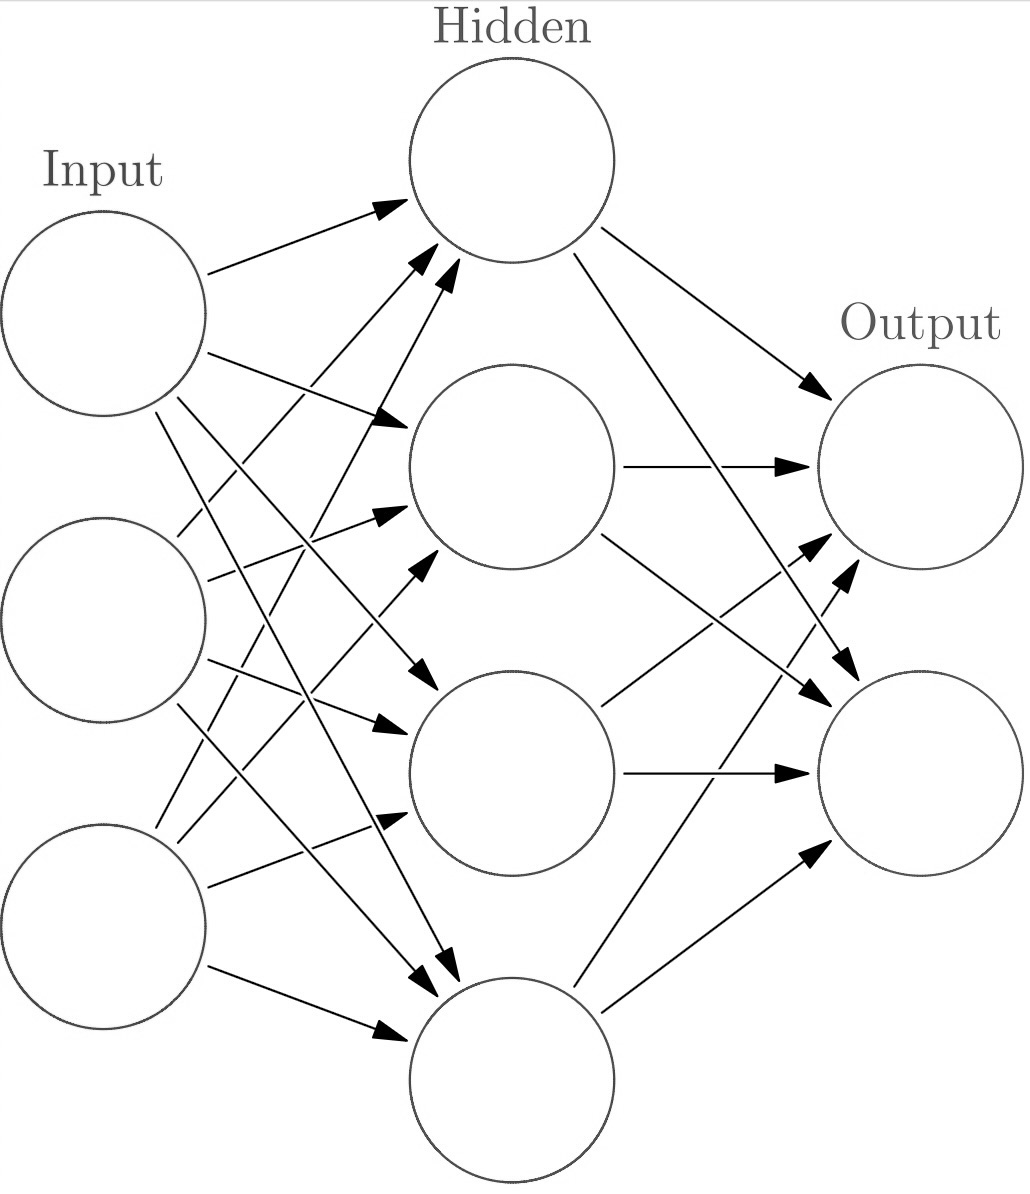
\includegraphics[width=0.5\textwidth]{figures/nn.jpeg}
  \caption{全连接神经网络}
  \label{fig:example}
\end{figure}

首先,我们选定网络每层的初始状态:

\begin{enumerate}
  \item 输入层:接受 $28\times28$ 的灰度图像作为输入,展平成784维的向量:
        \begin{equation}
          \mathbf{x} \in \mathbb{R}^{784}.
        \end{equation}

  \item 隐藏层:一个全连接层,包含50个神经元,激活函数为ReLU:
        \begin{equation}
          \mathbf{h} = \text{ReLU}(\mathbf{W}_1 \mathbf{x} + \mathbf{b}_1).
        \end{equation}
        其中,\(\mathbf{W}_1 \in \mathbb{R}^{50 \times 784}\) 为权重矩阵,\(\mathbf{b}_1 \in \mathbb{R}^{50}\) 为偏置向量。

  \item 输出层:一个全连接层,包含10个神经元,激活函数为Softmax:
        \begin{equation}
          \mathbf{y} = \text{Softmax}(\mathbf{W}_2 \mathbf{h} + \mathbf{b}_2).
        \end{equation}
        其中,\(\mathbf{W}_2 \in \mathbb{R}^{10 \times 50}\) 为权重矩阵,\(\mathbf{b}_2 \in \mathbb{R}^{10}\) 为偏置向量。
\end{enumerate}

约定这个神经网络中的符号如下表所示:

\begin{table}[htbp]
  \centering
  \caption{神经网络参数符号}
  \label{tab:nn}
  \begin{tabular}{cc}
    \toprule
    符号             & 含义           \\
    \midrule
    \(\mathbf{x}\)   & 输入向量       \\
    \(\mathbf{h}\)   & 隐藏层输出     \\
    \(\mathbf{y}\)   & 输出层输出     \\
    \(\mathbf{W}_1\) & 隐藏层权重矩阵 \\
    \(\mathbf{b}_1\) & 隐藏层偏置向量 \\
    \(\mathbf{W}_2\) & 输出层权重矩阵 \\
    \(\mathbf{b}_2\) & 输出层偏置向量 \\
    \bottomrule
  \end{tabular}
\end{table}

\subsubsection{训练过程}

训练该神经网络用到 60000 组学习数据和 10000 组测试数据,这些数据从 MNIST 数据集中导入,满足归一化条件,即 784 个像素的灰度值均用 $[0, 1]$ 区间内的实数表示。

令总迭代次数为 10000 次,每个 batch 包含 100 组学习数据,设定学习率为 0.1,然后开始训练。下图展示了训练过程中神经网络的准确率变化。

\begin{figure}[htbp]
  \centering
  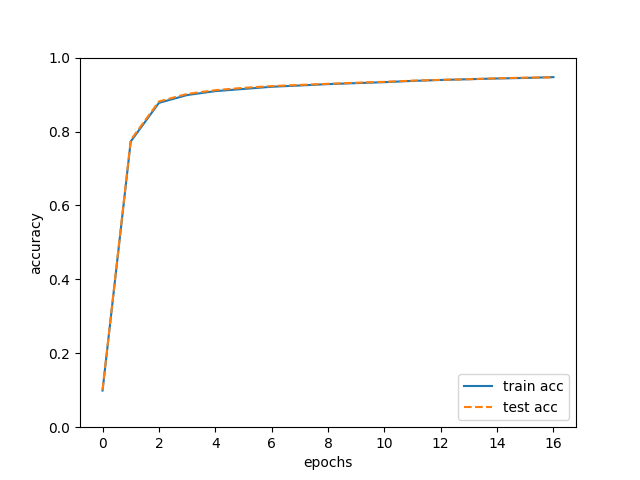
\includegraphics[width=1\textwidth]{figures/output.png}
  \caption{准确率变化折线图}
  \label{fig:nn_lyapunov_exponents}
\end{figure}

训练完成后,保存所有参数并在下一节中使用。

本文后续还将用到循环神经网络(RNN),RNN 的训练方法在此一并提及。

RNN 的训练可使用差值作为损失函数,并通过随机梯度下降法(SGD)对神经网络进行训练。具体步骤如下:

\begin{enumerate}
  \item 前向传播:计算每个时间步的隐藏状态和最终输出 \(\mathbf{y}\).
  \item 计算损失:使用差值作为损失函数 \(\mathcal{L}\).
  \item 反向传播:计算每层的梯度,并更新权重。在训练完成后,我们固定神经网络的参数,之后不再变动。
\end{enumerate}

\begin{equation}
  \mathbf{J}_t = \frac{\partial \mathbf{h}_t}{\partial \mathbf{h}_{t-1}}.
\end{equation}

\subsubsection{李雅普诺夫谱计算}

回到全连接神经网络,读取上一节保存的参数,使神经网络恢复到训练完成的状态。随机选取输入值 $x$ 和随机梯度,得到确定的状态 $x$、$h$、$y$ 和梯度 $\frac{\partial y}{\partial h}$、$\frac{\partial h}{\partial x}$.

矩阵 $Q_0$ 为随机矩阵 QR 分解后的结果,记 $v_0 = Q_0$,其含义为 10 个不同方向的输入层向量。

正向传播:

\begin{equation}
  \left\{
    \begin{aligned}
      v_1 &= \frac{\partial h}{\partial x} v_0 \\
      v_2 &= \frac{\partial y}{\partial h} v_1
    \end{aligned}
  \right.
\end{equation}

反向传播:

\begin{equation}
  \left\{
    \begin{aligned}
      \nu_1 &= \frac{\partial h}{\partial x} \nu_2 \\
      \nu_0 &= \frac{\partial y}{\partial h} \nu_1
    \end{aligned}
  \right.
\end{equation}

计算正向和反向传播的同时,使用算法 \ref{alg:lyapunov} 计算 $v$ 和 $\nu$ 在大量轨道(因输入数据不同)和大量 $\frac{v_0}{\nu_0}$ 意义下的李雅普诺夫谱。

全连接神经网络不能随时间无限延伸,正向和反向的传播均只进行两步,但可以通过多组输入来发现一般规律。

尝试 20 组不同的 $x$ 输入,得到 20 组不同的李雅普诺夫谱,每组有 10 个指数,由于网络长度有限,并且各层的宽度和结构不同,所以正向和反向的李雅普诺夫指数不能直接比较。但是他们各自的趋势仍有比较意义,也就是说正向和反向的李雅普诺夫谱会相差一个常数倍数。总体上呈现下降趋势:

\begin{figure}[htbp]
  \centering
  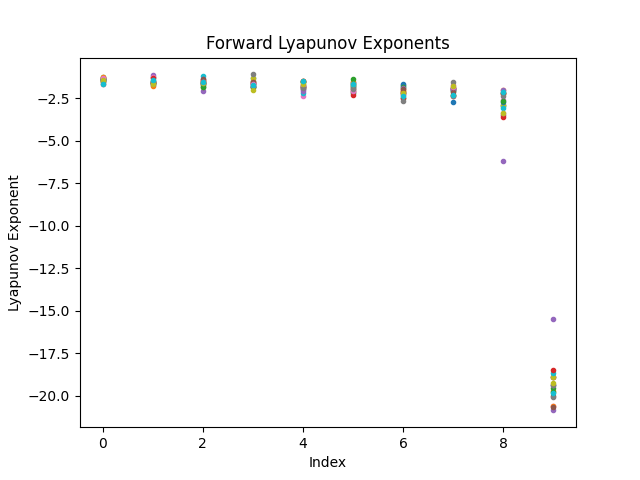
\includegraphics[width=1\textwidth]{figures/forward_lyapunov.png}
  \caption{正向传播的李雅普诺夫指数}
  \label{fig:nn_lyapunov_exponents}
\end{figure}

\begin{figure}[htbp]
  \centering
  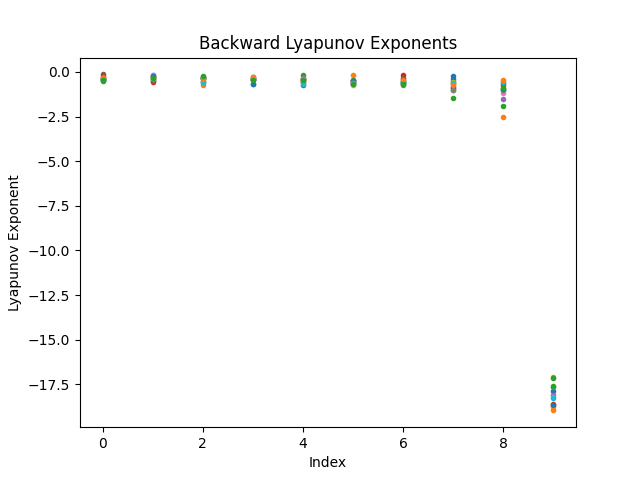
\includegraphics[width=1\textwidth]{figures/backward_lyapunov.png}
  \caption{反向传播的李雅普诺夫指数}
  \label{fig:nn_lyapunov_exponents}
\end{figure}

将多组数据取平均,得到如下散点图:

\begin{figure}[htbp]
  \centering
  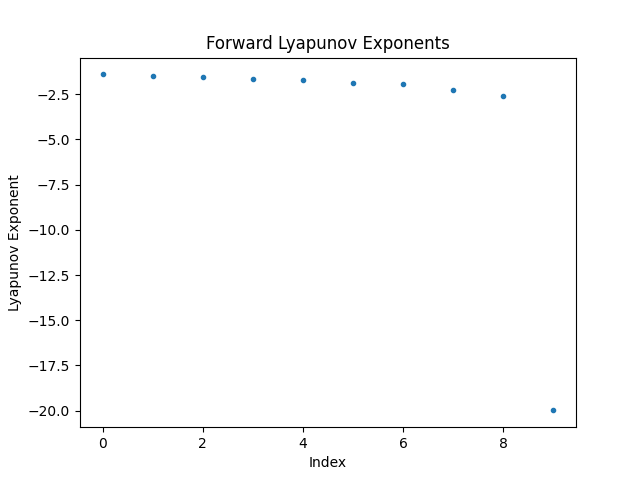
\includegraphics[width=1\textwidth]{figures/forward_lyapunov_avg.png}
  \caption{正向传播的平均李雅普诺夫指数}
  \label{fig:nn_lyapunov_exponents}
\end{figure}

\begin{figure}[htbp]
  \centering
  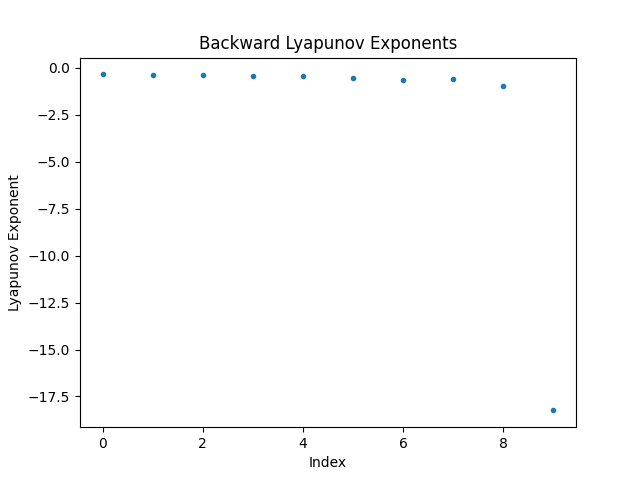
\includegraphics[width=1\textwidth]{figures/backward_lyapunov_avg.png}
  \caption{反向传播的平均李雅普诺夫指数}
  \label{fig:nn_lyapunov_exponents}
\end{figure}

\subsubsection{结果分析}

李雅普诺夫指数的个数由节点数目最少的输出层决定,在该网络中为 10 个。由上一小节的散点图,可以发现如下规律:

\begin{enumerate}
  \item 10 个李雅普诺夫指数均小于 0,说明该神经网络代表的动力系统是稳定的,不会出现梯度爆炸。
  \item 绝大多数方向的李雅普诺夫指数接近 0,意味着一般情况下,神经网络的梯度不会发生显著的梯度消失。
  \item $x=9$ 上的李雅普诺夫指数明显远小于其他方向,在这个方向上的梯度可能出现明显的梯度消失。
\end{enumerate}

至此已经完成了算法 \ref{alg:lyapunov} 的运行,但考虑到该全连接神经网络中间层的维数偏多,若验证对偶性将花费过长时间,因此我们将在下一节中考虑隐藏层维数较小的循环神经网络(RNN)。

\clearpage

\subsection{循环神经网络}\label{sec:rnn}

\subsubsection{网络结构}

RNN 在处理序列数据方面具有显著优势,能够捕捉时间步长上的依赖关系。在本实验中,我们选取一个循环神经网络(RNN),分别针对无输入、有输入的情形进行计算。选取任意时间步长 $T$,如下图示设计了一个简单的 RNN 模型,然后使用李雅普诺夫谱分析其动态行为。

和全连接神经网络类似,我们先尝试运行算法 \ref{alg:lyapunov},首先确定神经网络的参数规模和结构:

\begin{enumerate}
  \item 输入层:每个时间步的输入维度为 2
  \item 隐藏层:一个,隐藏状态维度为 3,激活函数为 tanh
  \item 输出层:维度为 2,激活函数为 Softmax
\end{enumerate}

\begin{figure}[htbp]
  \centering
  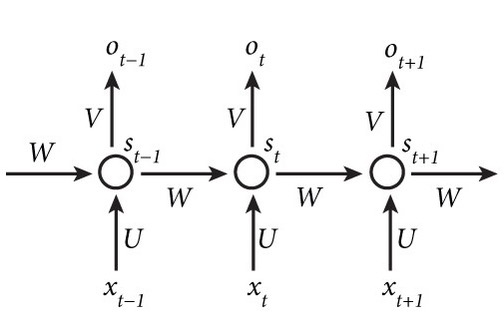
\includegraphics[width=0.5\textwidth]{figures/rnn.jpeg}
  \caption{循环神经网络}
  \label{fig:example}
\end{figure}

其次确定激活函数、权重矩阵和偏置向量:

\begin{enumerate}

  \item 输入层:每个时间步的输入维度为 2,时间步可任意长(在程序可计算的范围内)
        \begin{equation}
          \mathbf{x}_t \in \mathbb{R}^{3}.
        \end{equation}

  \item 隐藏层:一个 RNN 层,隐藏状态维度为 3,激活函数为 tanh:
        \begin{equation}
          \mathbf{h}_t = \text{tanh}(\mathbf{W}_{hh} \mathbf{h}_{t-1} + \mathbf{W}_{xh} \mathbf{x}_t + \mathbf{b}_h).
        \end{equation}
        其中,\(\mathbf{W}_{hh} \in \mathbb{R}^{3 \times 3}\) 和 \(\mathbf{W}_{xh} \in \mathbb{R}^{3 \times 3}\) 分别为隐藏状态和输入的权重矩阵,\(\mathbf{b}_h \in \mathbb{R}^{3}\) 为偏置向量。

  \item 输出层:维度为 3,激活函数为 Softmax:
        \begin{equation}
          \mathbf{y}_t = \text{Softmax}(\mathbf{W}_{hy} \mathbf{h}_t + \mathbf{b}_y).
        \end{equation}
        其中,\(\mathbf{W}_{hy} \in \mathbb{R}^{3 \times 3}\) 为权重矩阵,\(\mathbf{b}_y \in \mathbb{R}^{3}\) 为偏置向量。

\end{enumerate}

\subsubsection{李雅普诺夫谱计算}

计算正向传播的李雅普诺夫谱的具体算法如下:

\begin{algorithm}[H]
  \caption{计算 RNN 正向传播的 Lyapunov 谱}
  \begin{algorithmic}[1]
  \STATE 初始化 RNN,设定初始条件 $h_0$ 和输入序列 $x = \{x_t\}_{t=1}^T$.
  \STATE 随机生成 $m \times M$ 的正交矩阵 $Q_0$ 作为齐次切向解的初始条件。
  \FOR{$i = 0$ to $K - 1$}
      \STATE 计算 RNN 的隐藏状态 $h_i$ 和输出 $y_i$,$t \in [t_i, t_{i+1}]$.
      \STATE 计算齐次切向解 $W_i(t)$:
      \FOR{$j = 1$ to $M$}
          \STATE 从 $w_{ij}(t_i) = q_{ij}$ 积分方程到 $t_{i+1}$,该方程基于 RNN 的雅可比矩阵 $\frac{\partial h_{t+1}}{\partial h_t}$.
      \ENDFOR
      \STATE QR 分解:$W_i(t_{i+1}) = Q_{i+1} R_{i+1}$.
  \ENDFOR
  \STATE 计算李雅普诺夫指数 $\lambda_j$:
  \begin{equation}
  \lambda_j = \frac{1}{K \Delta T} \sum_{i=1}^K \log |D_{ij}|.
  \end{equation}
  其中 $D_{ij}$ 是 $R_i$ 的第 $j$ 个对角元素。
  \end{algorithmic}
\end{algorithm}

类似地,可以用如下算法计算反向传播的李雅普诺夫谱:

\begin{algorithm}[H]
  \caption{计算 RNN 反向传播的 Lyapunov 谱}
  \begin{algorithmic}[1]
  \STATE 初始化 RNN,设定初始条件 $h_0$ 和输入序列 $x = \{x_t\}_{t=1}^T$.
  \STATE 进行正向传播,计算每个时间步的隐藏状态 $h_t$ 和输出 $y_t$.
  \STATE 随机生成 $m \times M$ 的正交矩阵 $Q_T$ 作为齐次切向解的初始条件。
  \FOR{$i = T$ to $1$}
      \STATE 计算 RNN 的反向传播梯度 $\delta_i$,$t \in [t_i, t_{i-1}]$.
      \STATE 计算齐次切向解 $W_i(t)$:
      \FOR{$j = 1$ to $M$}
          \STATE 从 $w_{ij}(t_i) = q_{ij}$ 积分方程到 $t_{i-1}$,该方程基于 RNN 的雅可比矩阵 $\frac{\partial h_{t}}{\partial h_{t+1}}$.
      \ENDFOR
      \STATE QR 分解:$W_i(t_{i-1}) = Q_{i-1} R_{i-1}$.
  \ENDFOR
  \STATE 计算李雅普诺夫指数 $\lambda_j$:
  \begin{equation}
    \lambda_j = \frac{1}{K \Delta T} \sum_{i=1}^K \log |D_{ij}|.
  \end{equation}
  其中 $D_{ij}$ 是 $R_i$ 的第 $j$ 个对角元素。
  \end{algorithmic}
\end{algorithm}

\clearpage

\subsubsection{运行结果 - 无输入情形}

首先,简便起见,令输入序列 $\{x_t\}_{t=1}^T$ 全部为 0,即神经网络正向和反向的传播均不受到输入的影响。在此基础上尝试不同的 $T$ 值,以观察李雅普诺夫指数的收敛性。

三个方向的李雅普诺夫指数随 $T$ 的变化而变化,下图展示了迭代次数从 1 至 300 的正向李雅普诺夫指数变化规律:

\begin{figure}[htbp]
  \centering
  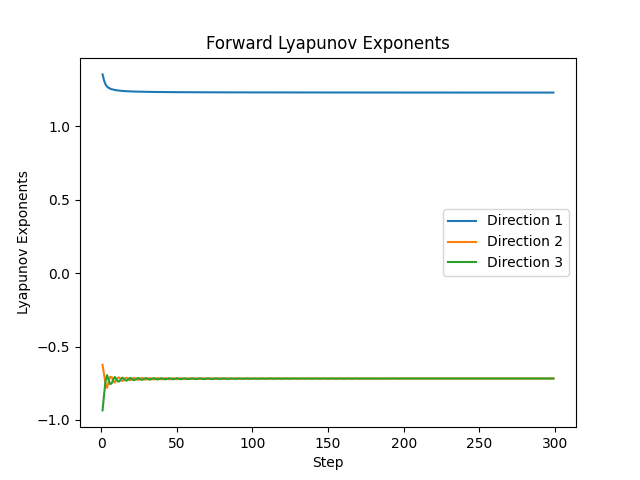
\includegraphics[width=0.7\textwidth]{figures/lyapunov_exponents_forward.png}
  \caption{正向传播收敛情况}
  \label{fig:example}
\end{figure}

由于不考虑输入的影响,反向的李雅普诺夫指数与正向相同:

\begin{figure}[htbp]
  \centering
  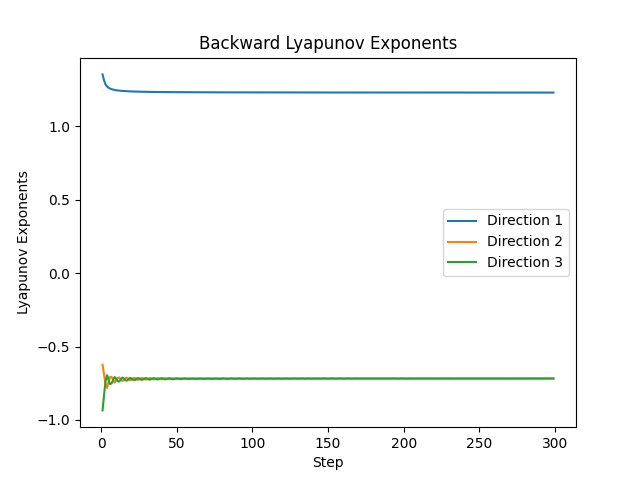
\includegraphics[width=0.7\textwidth]{figures/lyapunov_exponents_backward.png}
  \caption{反向传播收敛情况}
  \label{fig:example}
\end{figure}

在上面的算法中,我们取 $T=300$,运行程序。

实验结果显示,隐藏层的 3 个李雅普诺夫指数分别为:
\begin{equation}
  1.22852421\quad-0.71748841\quad-0.71789691
\end{equation}

根据运行结果显示,正向传播和反向传播的李雅普诺夫指数各自有一个大于 0,两个小于 0,其最大李雅普诺夫指数大于 0,从动力系统的角度分析,其最大李雅普诺夫指数大于 0,表明正向传播和反向传播的梯度不稳定,步数增多可能会导致梯度爆炸。

\subsubsection{运行结果 - 有输入情形}

下面我们进一步验证了有输入情形下的李雅普诺夫谱。我们将输入序列 $\{x_t\}_{t=1}^T$ 设置为随机生成的序列(numpy 的随机数种子设置为 42),以观察李雅普诺夫指数的变化。

运行 300 个时间步后得到的李雅普诺夫指数分别为:

\begin{enumerate}
  \item 正向:
  \begin{equation}
    0.00887475\quad-0.00384957\quad-0.00613681
  \end{equation}
  \item 反向:
  \begin{equation}
    0.00351433\quad-0.0024369\quad-0.00389064
  \end{equation}
\end{enumerate}

正向传播的 300 步的收敛过程如下图所示:

\begin{figure}[htbp]
  \centering
  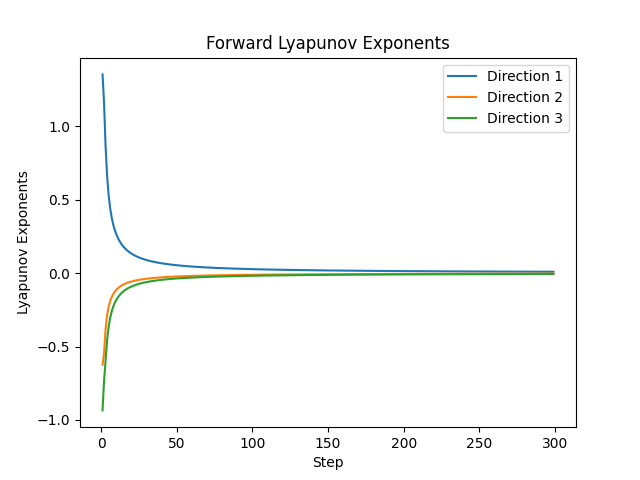
\includegraphics[width=0.7\textwidth]{figures/lyapunov_exponents_forward_with_input.png}
  \caption{有输入情形下的李雅普诺夫指数}
  \label{fig:example}
\end{figure}

反向传播的收敛过程与正向传播类似,且由于李雅普诺夫指数均十分接近 0,图像趋势没有太大区别。同时可以看到,随着 $T$ 的增加,正向和反向传播的李雅普诺夫指数均收敛,这表明前述算法对与一般情形的 RNN 同样有效。

经过对比,加入随机输入因素的前后有如下区别:

\begin{enumerate}
  \item 不考虑输入时,正反的李雅普诺夫谱数值相同,但有输入时,尽管两个李雅普诺夫谱均更接近 0,但二者不再相同。
  \item 加入随机输入后李雅普诺夫指数的绝对值变小,本文暂未找到明确的理论解释。
  \item 加入随机输入后李雅普诺夫指数随 $T$ 的收敛速度更快,对此同样暂没有明确的解释。
\end{enumerate}

虽然有种种不同,但下一节将验证,中间向量的对偶性依旧成立。

\subsection{对偶性的验证}\label{sec:duality}

对偶性的验证用到 \ref{sec:rnn_training} 中记录的中间向量,由算法 \ref{alg:lyapunov} 的原理,它们可以在计算李雅普诺夫谱的同时得到。将这些中间向量输出到日志文件中,然后读取并计算它们的内积,以验证对偶性。

下图形象展示了正向和反向传播的中间向量的内积,横轴表示时间步,可以发现,除去最边缘的极少数时间步,内积图像为一条直线,这表明正向和反向传播的中间向量的内积是一个常数,三条线的纵坐标即为三个方向对应的内积值。

\clearpage

\begin{figure}[htbp]
  \centering
  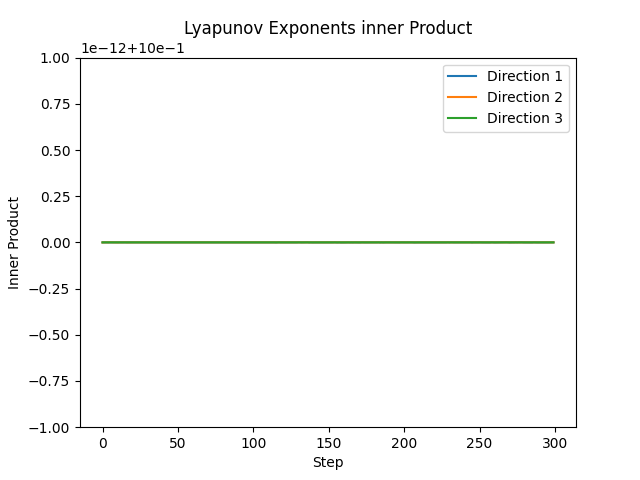
\includegraphics[width=0.7\textwidth]{figures/lyapunov_exponents_inner_product.png}
  \caption{无输入情形下的中间向量 $q_{ij}$ 内积}
  \label{fig:inner_product}
\end{figure}

由此我们便验证了正向传播和反向传播的中间向量 $q_{ij}$ 的有对偶性(不但内积固定,而且三个方向内积相同),但由于提前约定了输入为 0,仅能代表特殊情况,我们还需要进一步验证有输入情形下的对偶性。

使用相同方法,有输入时的中间向量内积如下图所示:

\clearpage

\begin{figure}[htbp]
  \centering
  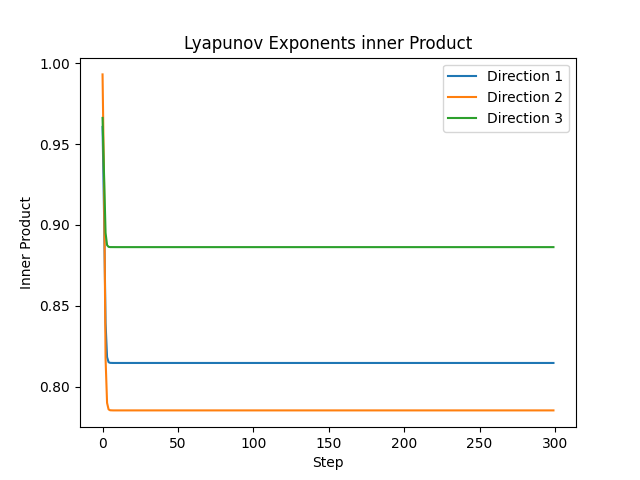
\includegraphics[width=0.7\textwidth]{figures/lyapunov_exponents_inner_product_with_input.png}
  \caption{有输入情形下的中间向量 $q_{ij}$ 内积}
  \label{fig:inner_product_with_input}
\end{figure}

有输入的情形下对偶性得到了保留,说明该性质与输入无关,是神经网络本身的特性,由其结构决定。

\section{结论}

本章深入探讨了不稳定神经网络的李雅普诺夫谱和中间向量的对偶性。通过详细的理论分析和实验验证,我们发现李雅普诺夫谱能够有效地揭示神经网络的动态特性,为网络的设计和优化提供了重要的理论支持,值得在未来的研究中进一步应用,此外,对偶性的验证也为神经网络的理论研究提供了新的视角,固定的内积值对于神经网络是否具有更多数学意义,值得进一步探讨。
% !TeX root = ../thuthesis-example.tex

\chapter{总结}

本文回顾了李雅普诺夫谱和李雅普诺夫指数,并介绍了计算李雅普诺夫指数的基本方法和应用。李雅普诺夫指数是用来描述一个动力系统中轨道对初始条件的敏感性的量度。在神经网络中,李雅普诺夫指数可以帮助我们理解网络的稳定性和动态行为。为了计算这些指数,本文采用了QR分解法,这是目前在计算李雅普诺夫谱中最为常用和有效的方法之一。

我们重点分析了在神经网络的训练过程中计算李雅普诺夫谱的表现。实验结果表明,李雅普诺夫指数可以作为一种有效的指标,用于评估网络的稳定性和预测训练过程中可能出现的数值问题。通过对李雅普诺夫指数的分析,我们可以提前发现并解决网络训练中的潜在问题,避免模型在训练后期出现不稳定或发散的现象。


% 其他部分
\backmatter

\listoffigures           % 插图清单
\listoftables            % 附表清单

% 参考文献
\bibliography{ref/refs}  % 参考文献使用 BibTeX 编译
% \printbibliography       % 参考文献使用 BibLaTeX 编译

% 致谢
% !TeX root = ../thuthesis-example.tex

\begin{acknowledgements}
总觉得来日方长,却不知岁月清浅,时节如流。当我提笔写下致谢时才发现,四年的大学生活即将结束,终于到了该说再见的时候了。四年的旅程,所有的相遇,所有的经历于我而言都是最好的礼物。愿走出校园的我们都会成为会更好的自己。

桃李不言,下自成蹊。在这次综合论文训练中,我最想要感谢的人是我的指导老师,倪昂修老师。相遇就是缘分,是良师亦是朋友,我想不到用什么华丽的语言来形容他,但是说起在做毕设和写论文过程中对我帮助最大的人,我第一时间想到的就是倪老师,从选题到中期,再到最终成文,他一直在很认真的指导我完成毕设和论文,并给出自己的建议,对于提出的的问题能够及时回复,除此之外,他还会关心我们的生活和工作,并给予一定的帮助和引导,是一位非常尽职尽责的老师涓涓师恩,铭记于心,感谢他帮助我完成了毕设和论文。我亦对于参与答辩工作的老师十分感激,感谢你们拨冗予以指导意见,让答辩对我显得尤为珍贵。

其次,我想感谢的是我的家人。我的家庭并非大富大贵之家,父母都是兢兢业业的教师,二十年来,对我的教育一直是包容胜过苛责,理解多于否定,在我心中,他们就是这个世界上最伟大的人,他们给了我生命,教会我成长,尊重我的选择,给予我无限的包容和关怀,是我最坚强的后盾。春晖寸草,难以回报,希望父母平安喜乐。

也感谢我的朋友,感谢你们在我写论文和毕设时给予的帮助。是你们陪伴我走过这四年的大学生涯,让平淡的生活增加了很多趣味,在我需要帮助时总是第-时间出现在我身边,让我在这四年感受到了很多的温暖和快乐,尤其感谢夏斐然同学,在大学四年里给我的生活带去了无穷乐趣。山河不足重,重在遇知己,祝大家前程似锦,在各自的领域闪闪发光。

最后我想感谢自己。我想对过去平凡且努力的自己说一声谢谢,这一路走来谈不上筚路蓝缕,但是也绝非易事,最让我引以为傲的事情就是一直在做自己,我们都应该活成自己喜欢的样子,做自己喜欢的事情,和喜欢的人交往,接受平凡的自己,也接受不完美的自己。

在走入社会后,希望自己永保初心,自由独立自信勇敢、不必羡慕谁,也不依附谁,做一个心中有光的人。宇宙山河烂漫,人间点滴温暖都值得我们继续前进。

行文至此,落笔为终。可以回头看,但不能走回头路,追风赶月莫停留,平芜尽处是春山,彼方尚有荣光在,愿我们前路漫漫亦灿灿。

\end{acknowledgements}


% 声明
% \statement
% 将签字扫描后的声明文件 scan-statement.pdf 替换原始页面
\statement[file=figures/scan-statement.pdf]
% 本科生编译生成的声明页默认不加页脚,插入扫描版时再补上;
% 研究生编译生成时有页眉页脚,插入扫描版时不再重复。
% 也可以手动控制是否加页眉页脚
% \statement[page-style=empty]
% \statement[file=scan-statement.pdf, page-style=plain]

% 附录
% 本科生需要将附录放到声明之后,个人简历之前
\appendix
% % !TeX root = ../thuthesis-example.tex

\begin{survey}
\label{cha:survey}

\title{Title of the Survey}
\maketitle


\tableofcontents


本科生的外文资料调研阅读报告。


\section{Figures and Tables}

\subsection{Figures}

An example figure in appendix (Figure~\ref{fig:appendix-survey-figure}).

\begin{figure}
  \centering
  \includegraphics[width=0.6\linewidth]{example-image-a.pdf}
  \caption{Example figure in appendix}
  \label{fig:appendix-survey-figure}
\end{figure}


\subsection{Tables}

An example table in appendix (Table~\ref{tab:appendix-survey-table}).

\begin{table}
  \centering
  \caption{Example table in appendix}
  \begin{tabular}{ll}
    \toprule
    File name       & Description                                         \\
    \midrule
    thuthesis.dtx   & The source file including documentaion and comments \\
    thuthesis.cls   & The template file                                   \\
    thuthesis-*.bst & BibTeX styles                                       \\
    thuthesis-*.bbx & BibLaTeX styles for bibliographies                  \\
    thuthesis-*.cbx & BibLaTeX styles for citations                       \\
    \bottomrule
  \end{tabular}
  \label{tab:appendix-survey-table}
\end{table}


\section{Equations}

An example equation in appendix (Equation~\eqref{eq:appendix-survey-equation}).
\begin{equation}
  \frac{1}{2 \uppi \symup{i}} \int_\gamma f = \sum_{k=1}^m n(\gamma; a_k) \mathscr{R}(f; a_k)
  \label{eq:appendix-survey-equation}
\end{equation}


\section{Citations}

Example citations in appendix.
\cite{abrahams99tex}
\cite{salomon1995advanced}
\cite{abrahams99tex,salomon1995advanced}


\bibliographystyle{unsrtnat}
\bibliography{ref/appendix}

\end{survey}
       % 本科生:外文资料的调研阅读报告
% % !TeX root = ../thuthesis-example.tex

\begin{translation}
\label{cha:translation}

\title{书面翻译题目}
\maketitle

\tableofcontents


本科生的外文资料书面翻译。


\section{图表示例}

\subsection{图}

附录中的图片示例(图~\ref{fig:appendix-translation-figure})。

\begin{figure}
  \centering
  \includegraphics[width=0.6\linewidth]{example-image-a.pdf}
  \caption{附录中的图片示例}
  \label{fig:appendix-translation-figure}
\end{figure}


\subsection{表格}

附录中的表格示例(表~\ref{tab:appendix-translation-table})。

\begin{table}
  \centering
  \caption{附录中的表格示例}
  \begin{tabular}{ll}
    \toprule
    文件名          & 描述                         \\
    \midrule
    thuthesis.dtx   & 模板的源文件,包括文档和注释 \\
    thuthesis.cls   & 模板文件                     \\
    thuthesis-*.bst & BibTeX 参考文献表样式文件    \\
    thuthesis-*.bbx & BibLaTeX 参考文献表样式文件  \\
    thuthesis-*.cbx & BibLaTeX 引用样式文件        \\
    \bottomrule
  \end{tabular}
  \label{tab:appendix-translation-table}
\end{table}


\section{数学公式}

附录中的数学公式示例(公式\eqref{eq:appendix-translation-equation})。
\begin{equation}
  \frac{1}{2 \uppi \symup{i}} \int_\gamma f = \sum_{k=1}^m n(\gamma; a_k) \mathscr{R}(f; a_k)
  \label{eq:appendix-translation-equation}
\end{equation}


\section{文献引用}

文献引用示例\cite{abrahams99tex}。


\appendix

\section{附录}

附录的内容。


% 书面翻译的参考文献
\bibliographystyle{unsrtnat}
\bibliography{ref/appendix}

% 书面翻译对应的原文索引
\begin{translation-index}
  \nocite{salomon1995advanced}
  \bibliographystyle{unsrtnat}
  \bibliography{ref/appendix}
\end{translation-index}

\end{translation}
  % 本科生:外文资料的书面翻译
% !TeX root = ../thuthesis-example.tex

\chapter{文献翻译}


% 个人简历、在学期间完成的相关学术成果
% 本科生可以附个人简历,也可以不附个人简历
% % !TeX root = ../thuthesis-example.tex

\begin{resume}

  \section*{个人简历}

  197× 年 ×× 月 ×× 日出生于四川××县。

  1992 年 9 月考入××大学化学系××化学专业,1996 年 7 月本科毕业并获得理学学士学位。

  1996 年 9 月免试进入清华大学化学系攻读××化学博士至今。


  \section*{在学期间完成的相关学术成果}

  \subsection*{学术论文}

  \begin{achievements}
    \item Yang Y, Ren T L, Zhang L T, et al. Miniature microphone with silicon-based ferroelectric thin films[J]. Integrated Ferroelectrics, 2003, 52:229-235.
    \item 杨轶, 张宁欣, 任天令, 等. 硅基铁电微声学器件中薄膜残余应力的研究[J]. 中国机械工程, 2005, 16(14):1289-1291.
    \item 杨轶, 张宁欣, 任天令, 等. 集成铁电器件中的关键工艺研究[J]. 仪器仪表学报, 2003, 24(S4):192-193.
    \item Yang Y, Ren T L, Zhu Y P, et al. PMUTs for handwriting recognition. In press[J]. (已被Integrated Ferroelectrics录用)
  \end{achievements}


  \subsection*{专利}

  \begin{achievements}
    \item 任天令, 杨轶, 朱一平, 等. 硅基铁电微声学传感器畴极化区域控制和电极连接的方法: 中国, CN1602118A[P]. 2005-03-30.
    \item Ren T L, Yang Y, Zhu Y P, et al. Piezoelectric micro acoustic sensor based on ferroelectric materials: USA, No.11/215, 102[P]. (美国发明专利申请号.)
  \end{achievements}

\end{resume}


% 指导教师/指导小组评语
% 本科生不需要
% % !TeX root = ../thuthesis-example.tex

\begin{comments}
% \begin{comments}[name = {指导小组评语}]
% \begin{comments}[name = {Comments from Thesis Supervisor}]
% \begin{comments}[name = {Comments from Thesis Supervision Committee}]

  论文提出了……

\end{comments}


% 答辩委员会决议书
% 本科生不需要
% % !TeX root = ../thuthesis-example.tex

\begin{resolution}

  论文提出了……

  论文取得的主要创新性成果包括:

  1. ……

  2. ……

  3. ……

  论文工作表明作者在×××××具有×××××知识,具有××××能力,论文××××,答辩××××。

  答辩委员会表决,(×票/一致)同意通过论文答辩,并建议授予×××(姓名)×××(门类)学博士/硕士学位。

\end{resolution}


% 本科生的综合论文训练记录表(扫描版)
% \record{file=scan-record.pdf}

\end{document}
